\documentclass[11pt,a4paper,openany]{ctexbook}
\usepackage[margin=2.1cm,headheight=16pt]{geometry}
\usepackage{amsmath,amssymb,mathtools,bm}
\usepackage{graphicx}
\usepackage{fontspec}
\IfFontExistsTF{Noto Serif CJK SC}{%
  \setCJKmainfont{Noto Serif CJK SC}%
  \setCJKsansfont{Noto Sans CJK SC}%
  \IfFontExistsTF{Noto Sans Mono CJK SC}{\setCJKmonofont{Noto Sans Mono CJK SC}}{}%
}{}
\usepackage{enumitem}
\usepackage{booktabs,tabularx,longtable,array,multicol}
\usepackage{xcolor}
\usepackage[most]{tcolorbox}
\usepackage{tikz}
\usetikzlibrary{calc,intersections,angles,quotes,arrows.meta,positioning,decorations.pathreplacing}
\usepackage{fancyhdr}
\usepackage{titlesec}
\usepackage{hyperref}
\usepackage{needspace}
\usepackage{lastpage}
\let\cleardoublepage\clearpage
\hypersetup{colorlinks=true,linkcolor=blue!45!black,urlcolor=blue!55!black}

\definecolor{navy}{HTML}{17365D}
\definecolor{bluegray}{HTML}{EAF1F8}
\definecolor{teal}{HTML}{0F6B78}
\definecolor{gold}{HTML}{C58A17}
\definecolor{softgold}{HTML}{FFF7DF}
\definecolor{softgreen}{HTML}{EAF6F0}
\definecolor{softred}{HTML}{FCEEEE}
\definecolor{ink}{HTML}{23262B}

\pagestyle{fancy}
\fancyhf{}
\fancyhead[L]{\color{navy}\small 高中数学·平面向量图解教案}
\fancyhead[R]{\color{gray}\small \leftmark}
\fancyfoot[C]{\small 第 \thepage\ 页}
\renewcommand{\headrulewidth}{0.4pt}
\renewcommand{\footrulewidth}{0pt}

\setcounter{secnumdepth}{-1}
\titleformat{\chapter}[display]
  {\bfseries\sffamily\color{navy}}
  {}
  {0pt}
  {\titlerule[1.2pt]\vspace{0.8ex}\Huge}
\titleformat{\section}{\Large\bfseries\sffamily\color{teal}}{}{0pt}{}
\titleformat{\subsection}{\large\bfseries\sffamily\color{navy}}{}{0pt}{}

\setlength{\parindent}{2em}
\setlength{\parskip}{0.25em}
\linespread{1.22}
\setlist[itemize]{leftmargin=2em,itemsep=0.25em,topsep=0.35em}
\setlist[enumerate]{leftmargin=2.3em,itemsep=0.35em,topsep=0.35em}

\newtcolorbox{teachbox}[1][]{breakable,colback=bluegray,colframe=navy!70!black,
  boxrule=0.7pt,arc=2mm,left=2mm,right=2mm,top=1.5mm,bottom=1.5mm,
  title={教学设计},fonttitle=\bfseries\sffamily,#1}
\newtcolorbox{theorembox}[1]{breakable,colback=softgreen,colframe=teal,
  boxrule=0.8pt,arc=2mm,title={#1},fonttitle=\bfseries\sffamily}
\newtcolorbox{warningbox}[1][]{breakable,colback=softred,colframe=red!55!black,
  boxrule=0.7pt,arc=2mm,title={易错警报},fonttitle=\bfseries\sffamily,#1}
\newtcolorbox{methodbox}[1][]{breakable,colback=softgold,colframe=gold!80!black,
  boxrule=0.7pt,arc=2mm,title={方法提炼},fonttitle=\bfseries\sffamily,#1}
\newtcolorbox{problem}[1]{breakable,colback=white,colframe=navy!65,
  boxrule=0.75pt,arc=1.5mm,title={#1},fonttitle=\bfseries\sffamily,
  before skip=0.8em,after skip=0.4em}
\newtcolorbox{solution}{breakable,colback=gray!3,colframe=gray!45,
  boxrule=0.55pt,arc=1.5mm,title={解析},fonttitle=\bfseries\sffamily,
  before skip=0.2em,after skip=0.8em}
\newtcolorbox{summarybox}[1]{breakable,colback=white,colframe=teal!70,
  boxrule=0.9pt,arc=2mm,title={#1},fonttitle=\bfseries\sffamily}

\newcommand{\vect}[1]{\overrightarrow{#1}}
\newcommand{\vv}[1]{\bm{#1}}
\newcommand{\dotp}{\mathbin{\boldsymbol\cdot}}
\newcommand{\src}[1]{\par\hfill{\footnotesize\color{gray}来源：#1}}
\newcommand{\ans}[1]{\par\noindent\textbf{答案：}\( #1 \)}
\newcommand{\R}{\mathbb{R}}
\newcommand{\area}[1]{S_{\triangle #1}}
\newcommand{\circled}[1]{\tikz[baseline=(char.base)]{\node[shape=circle,draw,inner sep=1pt,font=\scriptsize] (char) {#1};}}

% ---------- Diagram system ----------
\tikzset{
  geom/.style={draw=navy!82,line width=.85pt},
  vline/.style={-{Stealth[length=2.2mm,width=1.5mm]},draw=teal,line width=1pt},
  hline/.style={draw=gold!90!black,line width=1.15pt},
  aid/.style={draw=gray!65,dashed,line width=.65pt},
  vpoint/.style={circle,fill=navy,inner sep=1.35pt},
  moving/.style={circle,fill=gold!90!black,inner sep=1.55pt},
  centerpt/.style={circle,fill=teal,inner sep=1.55pt},
  faint/.style={fill=teal!9,draw=teal!45},
  regionA/.style={fill=teal!13,draw=none},
  regionB/.style={fill=gold!15,draw=none},
  regionC/.style={fill=blue!8,draw=none}
}
\newcommand{\figcap}[2]{%
  \begin{center}\begin{minipage}{.92\linewidth}\centering
  \ifx&#1&\else#1\fi
  \ifx&#2&\else\ifx&#1&\else\\[-.35em]\fi{\footnotesize\color{gray}#2}\fi
  \end{minipage}\end{center}}

\newcommand{\figVectorLanguage}{%
\begin{tikzpicture}[scale=.78,every node/.style={font=\small}]
  \coordinate (A) at (0,0); \coordinate (B) at (2.1,1.0);
  \coordinate (C) at (3.2,-.1); \coordinate (D) at (5.3,.9);
  \draw[vline] (A)--(B) node[midway,above left] {$\vec a$};
  \draw[vline] (C)--(D) node[midway,above left] {$\vec a$};
  \draw[vline,draw=gold!90!black] (B)--(A) node[midway,below right] {$-\vec a$};
  \node[vpoint,label=below:$A$] at (A){}; \node[vpoint,label=above:$B$] at (B){};
  \node[vpoint,label=below:$C$] at (C){}; \node[vpoint,label=above:$D$] at (D){};
  \node[align=center,text=gray!80!black] at (2.65,1.65) {位置不同不影响向量相等};
\end{tikzpicture}}

\newcommand{\figVectorAdd}{%
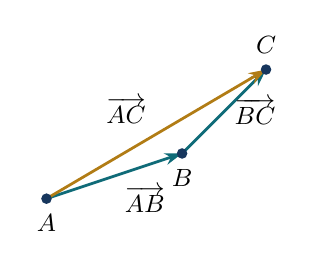
\begin{tikzpicture}[scale=.82,every node/.style={font=\small}]
  \coordinate (A) at (0,0); \coordinate (B) at (2.1,.7); \coordinate (C) at (3.4,2.0);
  \draw[vline] (A)--(B) node[midway,below right] {$\overrightarrow{AB}$};
  \draw[vline] (B)--(C) node[midway,right] {$\overrightarrow{BC}$};
  \draw[vline,draw=gold!90!black] (A)--(C) node[midway,above left] {$\overrightarrow{AC}$};
  \node[vpoint,label=below:$A$] at (A){}; \node[vpoint,label=below:$B$] at (B){}; \node[vpoint,label=above:$C$] at (C){};
\end{tikzpicture}}

\newcommand{\figBasis}{%
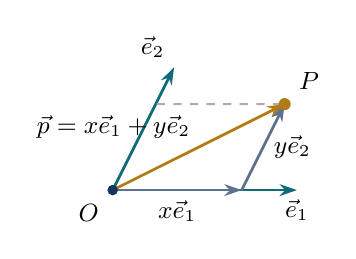
\begin{tikzpicture}[scale=.78,every node/.style={font=\small}]
  \coordinate (O) at (0,0); \coordinate (E1) at (3,0); \coordinate (E2) at (1.0,2.0);
  \coordinate (X) at (2.1,0); \coordinate (Y) at (.7,1.4); \coordinate (P) at (2.8,1.4);
  \draw[vline] (O)--(E1); \node[below] at (E1) {$\vec e_1$};
  \draw[vline] (O)--(E2); \node[above left] at (E2) {$\vec e_2$};
  \draw[vline,draw=gold!90!black] (O)--(P) node[midway,above left=-1pt] {$\vec p=x\vec e_1+y\vec e_2$};
  \draw[aid] (X)--(P)--(Y);
  \draw[vline,draw=navy!70] (O)--(X) node[midway,below] {$x\vec e_1$};
  \draw[vline,draw=navy!70] (X)--(P) node[midway,right] {$y\vec e_2$};
  \node[vpoint,label=below left:$O$] at (O){}; \node[moving,label=above right:$P$] at (P){};
\end{tikzpicture}}

\newcommand{\figDivision}{%
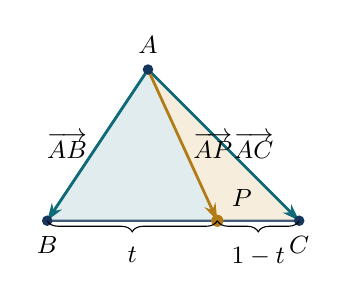
\begin{tikzpicture}[scale=.8,every node/.style={font=\small}]
  \coordinate (A) at (1.6,2.4); \coordinate (B) at (0,0); \coordinate (C) at (4,0); \coordinate (P) at (2.7,0);
  \fill[regionA] (A)--(B)--(P)--cycle; \fill[regionB] (A)--(P)--(C)--cycle;
  \draw[geom] (A)--(B)--(C)--cycle;
  \draw[vline] (A)--(B) node[midway,left] {$\overrightarrow{AB}$};
  \draw[vline] (A)--(C) node[midway,right] {$\overrightarrow{AC}$};
  \draw[vline,draw=gold!90!black] (A)--(P) node[midway,right] {$\overrightarrow{AP}$};
  \node[vpoint,label=above:$A$] at (A){}; \node[vpoint,label=below:$B$] at (B){}; \node[vpoint,label=below:$C$] at (C){}; \node[moving,label=above right:$P$] at (P){};
  \draw[decorate,decoration={brace,amplitude=4pt,mirror}] (B)--(P) node[midway,below=6pt] {$t$};
  \draw[decorate,decoration={brace,amplitude=4pt,mirror}] (P)--(C) node[midway,below=6pt] {$1-t$};
\end{tikzpicture}}

\newcommand{\figInterceptRatio}{%
\begin{tikzpicture}[scale=.75,every node/.style={font=\small}]
  \coordinate (A) at (0,0); \coordinate (B0) at (2.5,0); \coordinate (C0) at (0.4,1.2);
  \coordinate (Bk) at (3.75,0); \coordinate (Ck) at (0.6,1.8);
  \coordinate (P) at (2.4,0.7714);
  \draw[geom] (A)--(4.2,0); \draw[geom] (A)--(0.8,2.4);
  \draw[aid,dashed,thick] (B0)--(C0) node[midway,below left,font=\scriptsize,text=gray!80!black] {基线 \(L_1(k=1)\)};
  \draw[hline] (-0.2,2.257)--(4.25,-0.286) node[right,font=\scriptsize,text=gold!90!black] {平行等和线 \(L_k: a\lambda+b\mu=k\)};
  \draw[vline,draw=gold!90!black] (A)--(P);
  \node[vpoint,label=below left:$A$] at (A){};
  \node[vpoint,label=below:$B_0$] at (B0){}; \node[vpoint,label=left:$C_0$] at (C0){};
  \node[vpoint,label=below:$B_k$] at (Bk){}; \node[vpoint,label=left:$C_k$] at (Ck){};
  \node[moving,label=above right:$P$] at (P){};
\end{tikzpicture}}
\newcommand{\figProjectionDot}{%
\begin{tikzpicture}[scale=.78,every node/.style={font=\small}]
  \coordinate (A) at (0,0); \coordinate (B) at (2.4,0); \coordinate (C) at (0.6,2.0);
  \coordinate (P) at (2.8,1.8);
  \coordinate (M) at (1.2,0.32);
  \coordinate (Pproj) at (3.0,0.8);
  \draw[geom] (A)--(B); \draw[geom] (A)--(C);
  \draw[vline,draw=gold!90!black] (A)--(P);
  \draw[aid,dashed] (A)--(3.8,1.013) node[right,font=\scriptsize,text=gray!70!black] {\(\vec m\) 方向轴};
  \draw[thick,draw=teal] (A)--(Pproj) node[midway,below right=2pt,font=\scriptsize,text=teal] {投影 \(AP'\)};
  \draw[aid,->,>=stealth,draw=teal,ultra thick] (A)--(M) node[midway,above left=1pt,font=\scriptsize,text=teal] {辅助向量 \(\vec m\)};
  \draw[aid,dashed,draw=teal] (P)--(Pproj);
  \node[vpoint,label=below left:$A$] at (A){}; \node[vpoint,label=below:$B$] at (B){}; \node[vpoint,label=left:$C$] at (C){};
  \node[moving,label=above right:$P$] at (P){}; \node[vpoint,label=below right:$P'$] at (Pproj){};
\end{tikzpicture}}
\newcommand{\figEqualSumGeneral}{%
\begin{tikzpicture}[scale=.78,every node/.style={font=\small}]
  \coordinate (A) at (0,0); \coordinate (B) at (2.0,0); \coordinate (C) at (0.8,2.0);
  \coordinate (Q) at (1.2,3.0); \coordinate (P) at (2.64,0.6);
  \draw[geom] (A)--(B); \draw[geom] (A)--(C);
  \draw[aid] (B)--(C) node[midway,above right,font=\scriptsize,text=gray!70!black] {基线 \(BC\) (\(\lambda+\mu=1\))};
  \draw[hline] (-0.3,5.5)--(3.3,-0.5) node[right,font=\scriptsize,text=gold!90!black] {等和轨迹线 \(\lambda+\mu=k \parallel BC\)};
  \draw[vline,draw=gold!90!black] (A)--(P);
  \draw[aid,draw=teal,->,>=stealth] (Q)--(P) node[midway,above right,font=\scriptsize,text=teal] {\(\lambda\vect{CB}\)};
  \draw[aid] (C)--(Q);
  \node[vpoint,label=below left:$A$] at (A){}; \node[vpoint,label=below:$B$] at (B){}; \node[vpoint,label=left:$C$] at (C){};
  \node[vpoint,label=above left:$Q$] at (Q){}; \node[moving,label=right:$P$] at (P){};
\end{tikzpicture}}
\newcommand{\figEqualSum}{%
\begin{tikzpicture}[scale=.75,every node/.style={font=\small}]
  \coordinate (O) at (0,0); \coordinate (A) at (2.0,0); \coordinate (B) at (1.414,1.414);
  \coordinate (A1) at (3.0,0); \coordinate (B1) at (4.242,4.242);
  \coordinate (P) at (2.121,1.414);
  \draw[geom] (O)--(A); \draw[geom] (O)--(B);
  \draw[hline] (-0.3,5.1)--(4.5,-0.6) node[right,font=\scriptsize,text=gold!90!black] {等和轨迹线 \(2\lambda+\mu=3\)};
  \draw[vline,draw=gold!90!black] (O)--(P);
  \node[vpoint,label=below left:$O$] at (O){}; \node[vpoint,label=below:$A$] at (A){}; \node[vpoint,label=above left:$B$] at (B){};
  \node[vpoint,label=below:$A'$] at (A1){}; \node[vpoint,label=above right:$B'$] at (B1){}; \node[moving,label=above right:$P_{\min}$] at (P){};
\end{tikzpicture}}

\newcommand{\figIntercept}{%
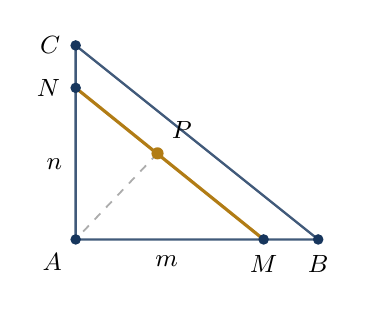
\begin{tikzpicture}[scale=.77,every node/.style={font=\small}]
  \coordinate (A) at (0,0); \coordinate (B) at (4,0); \coordinate (C) at (0,3.2);
  \coordinate (M) at (3.1,0); \coordinate (N) at (0,2.5); \coordinate (P) at (1.35,1.42);
  \draw[geom] (A)--(B)--(C)--cycle;
  \draw[hline] (M)--(N);
  \draw[aid] (P)--(A);
  \node[vpoint,label=below left:$A$] at (A){}; \node[vpoint,label=below:$B$] at (B){}; \node[vpoint,label=left:$C$] at (C){};
  \node[vpoint,label=below:$M$] at (M){}; \node[vpoint,label=left:$N$] at (N){}; \node[moving,label=above right:$P$] at (P){};
  \node at (1.5,-.35) {$m$}; \node at (-.35,1.25) {$n$};
\end{tikzpicture}}

\newcommand{\figCevian}{%
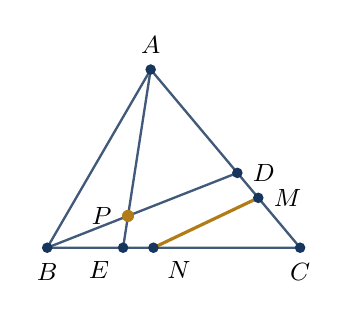
\begin{tikzpicture}[scale=.73,every node/.style={font=\small}]
  \coordinate (A) at (1.8,3.1); \coordinate (B) at (0,0); \coordinate (C) at (4.4,0);
  \coordinate (D) at ($(A)!.58!(C)$); \coordinate (E) at ($(B)!.30!(C)$);
  \path[name path=BD] (B)--(D); \path[name path=AE] (A)--(E);
  \path[name intersections={of=BD and AE,by=P}];
  \coordinate (M) at ($(A)!.72!(C)$); \coordinate (N) at ($(B)!.42!(C)$);
  \draw[geom] (A)--(B)--(C)--cycle;
  \draw[geom] (B)--(D); \draw[geom] (A)--(E); \draw[hline] (M)--(N);
  \node[vpoint,label=above:$A$] at (A){}; \node[vpoint,label=below:$B$] at (B){}; \node[vpoint,label=below:$C$] at (C){};
  \node[vpoint,label=right:$D$] at (D){}; \node[vpoint,label=below left:$E$] at (E){}; \node[moving,label=left:$P$] at (P){};
  \node[vpoint,label=right:$M$] at (M){}; \node[vpoint,label=below right:$N$] at (N){};
\end{tikzpicture}}

\newcommand{\figDP}{%
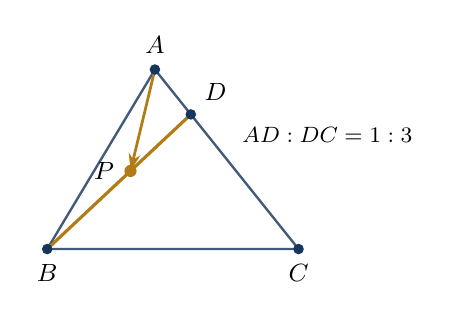
\begin{tikzpicture}[scale=.76,every node/.style={font=\small}]
  \coordinate (A) at (1.8,3); \coordinate (B) at (0,0); \coordinate (C) at (4.2,0);
  \coordinate (D) at ($(A)!.25!(C)$); \coordinate (P) at ($(B)!.58!(D)$);
  \draw[geom] (A)--(B)--(C)--cycle; \draw[hline] (B)--(D); \draw[vline,draw=gold!90!black] (A)--(P);
  \node[vpoint,label=above:$A$] at (A){}; \node[vpoint,label=below:$B$] at (B){}; \node[vpoint,label=below:$C$] at (C){};
  \node[vpoint,label=above right:$D$] at (D){}; \node[moving,label=left:$P$] at (P){};
  \node[font=\footnotesize,anchor=west] at (3.1,1.9) {$AD:DC=1:3$};
\end{tikzpicture}}

\newcommand{\figCentroidCross}{%
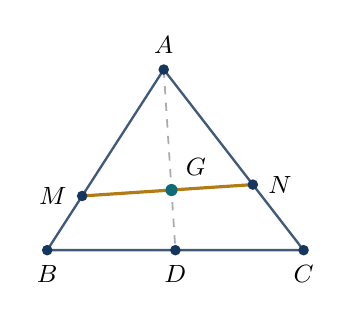
\begin{tikzpicture}[scale=.74,every node/.style={font=\small}]
  \coordinate (A) at (2,3.1); \coordinate (B) at (0,0); \coordinate (C) at (4.4,0); \coordinate (D) at (2.2,0);
  \coordinate (G) at ($(A)!.667!(D)$); \coordinate (M) at ($(A)!.70!(B)$);
  \path[name path=ad] (A)--(D); \path[name path=mg] (M)--($(M)!2.5!(G)$);
  \path[name path=ac] (A)--(C); \path[name intersections={of=mg and ac,by=N}];
  \draw[geom] (A)--(B)--(C)--cycle; \draw[aid] (A)--(D); \draw[hline] (M)--(N);
  \node[vpoint,label=above:$A$] at (A){}; \node[vpoint,label=below:$B$] at (B){}; \node[vpoint,label=below:$C$] at (C){}; \node[vpoint,label=below:$D$] at (D){};
  \node[centerpt,label=above right:$G$] at (G){}; \node[vpoint,label=left:$M$] at (M){}; \node[vpoint,label=right:$N$] at (N){};
\end{tikzpicture}}

\newcommand{\figDOnAB}{%
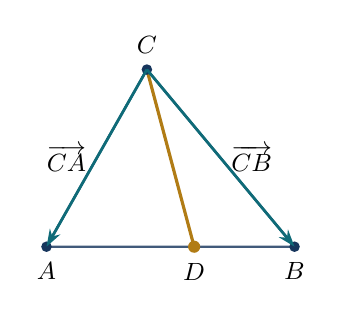
\begin{tikzpicture}[scale=.75,every node/.style={font=\small}]
  \coordinate (A) at (0,0); \coordinate (B) at (4.2,0); \coordinate (C) at (1.7,3); \coordinate (D) at (2.5,0);
  \draw[geom] (A)--(B)--(C)--cycle; \draw[hline] (C)--(D);
  \node[vpoint,label=below:$A$] at (A){}; \node[vpoint,label=below:$B$] at (B){}; \node[vpoint,label=above:$C$] at (C){}; \node[moving,label=below:$D$] at (D){};
  \draw[vline] (C)--(A) node[midway,left] {$\overrightarrow{CA}$};
  \draw[vline] (C)--(B) node[midway,right] {$\overrightarrow{CB}$};
\end{tikzpicture}}

\newcommand{\figMedianCross}{%
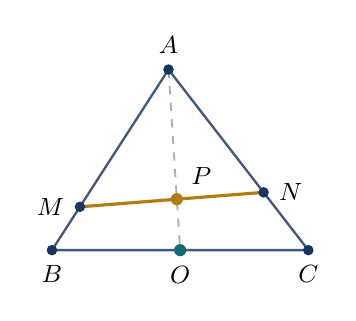
\begin{tikzpicture}[scale=.74,every node/.style={font=\small}]
  \coordinate (A) at (2,3.1); \coordinate (B) at (0,0); \coordinate (C) at (4.4,0); \coordinate (O) at (2.2,0);
  \coordinate (M) at ($(A)!.76!(B)$); \coordinate (N) at ($(A)!.68!(C)$);
  \path[name path=ao] (A)--(O); \path[name path=mn] (M)--(N);
  \path[name intersections={of=ao and mn,by=P}];
  \draw[geom] (A)--(B)--(C)--cycle; \draw[aid] (A)--(O); \draw[hline] (M)--(N);
  \node[vpoint,label=above:$A$] at (A){}; \node[vpoint,label=below:$B$] at (B){}; \node[vpoint,label=below:$C$] at (C){};
  \node[centerpt,label=below:$O$] at (O){}; \node[moving,label=above right:$P$] at (P){}; \node[vpoint,label=left:$M$] at (M){}; \node[vpoint,label=right:$N$] at (N){};
\end{tikzpicture}}

\newcommand{\figComplexCevian}{%
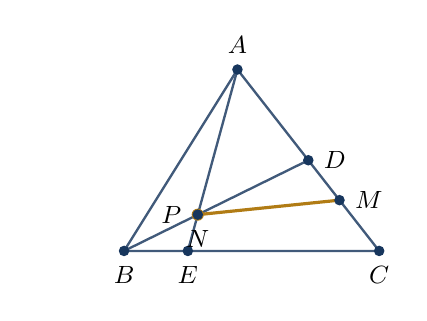
\begin{tikzpicture}[scale=.72,every node/.style={font=\small}]
  \coordinate (A) at (2,3.2); \coordinate (B) at (0,0); \coordinate (C) at (4.5,0);
  \coordinate (D) at ($(A)!.5!(C)$); \coordinate (E) at ($(B)!.25!(C)$);
  \path[name path=bd] (B)--(D); \path[name path=ae] (A)--(E); \path[name intersections={of=bd and ae,by=P}];
  \coordinate (M) at ($(A)!.72!(C)$);
  \path[name path=mp] (M)--($(M)!2.2!(P)$); \path[name path=bc] (B)--(C);
  \path[name intersections={of=mp and bc,by=N}];
  \draw[geom] (A)--(B)--(C)--cycle; \draw[geom] (B)--(D) (A)--(E); \draw[hline] (M)--(N);
  \node[vpoint,label=above:$A$] at (A){}; \node[vpoint,label=below:$B$] at (B){}; \node[vpoint,label=below:$C$] at (C){};
  \node[vpoint,label=right:$D$] at (D){}; \node[vpoint,label=below:$E$] at (E){}; \node[moving,label=left:$P$] at (P){};
  \node[vpoint,label=right:$M$] at (M){}; \node[vpoint,label=below:$N$] at (N){};
\end{tikzpicture}}

\newcommand{\figScaledE}{%
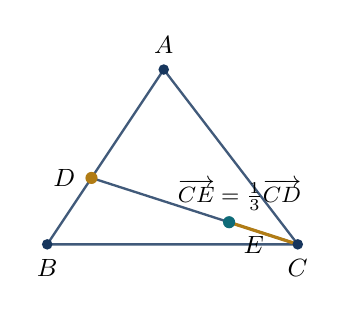
\begin{tikzpicture}[scale=.74,every node/.style={font=\small}]
  \coordinate (A) at (2,3); \coordinate (B) at (0,0); \coordinate (C) at (4.3,0); \coordinate (D) at ($(A)!.62!(B)$); \coordinate (E) at ($(C)!.333!(D)$);
  \draw[geom] (A)--(B)--(C)--cycle; \draw[geom] (C)--(D); \draw[hline] (C)--(E);
  \node[vpoint,label=above:$A$] at (A){}; \node[vpoint,label=below:$B$] at (B){}; \node[vpoint,label=below:$C$] at (C){}; \node[moving,label=left:$D$] at (D){}; \node[centerpt,label=below right:$E$] at (E){};
  \node[font=\footnotesize] at (3.3,.85) {$\overrightarrow{CE}=\frac13\overrightarrow{CD}$};
\end{tikzpicture}}

\newcommand{\figTwoCevianExact}{%
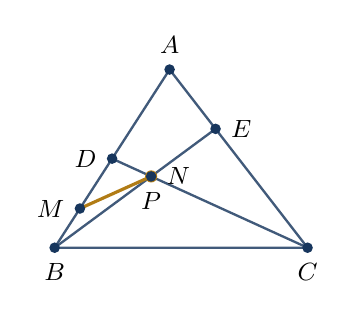
\begin{tikzpicture}[scale=.73,every node/.style={font=\small}]
  \coordinate (A) at (2,3.1); \coordinate (B) at (0,0); \coordinate (C) at (4.4,0);
  \coordinate (D) at ($(A)!.5!(B)$); \coordinate (E) at ($(A)!.333!(C)$);
  \path[name path=cd] (C)--(D); \path[name path=be] (B)--(E); \path[name intersections={of=cd and be,by=P}];
  \coordinate (M) at ($(A)!.78!(B)$);
  \path[name path=mp] (M)--($(M)!1.8!(P)$); \path[name path=ac] (A)--(C);
  \path[name intersections={of=mp and ac,by=N}];
  \draw[geom] (A)--(B)--(C)--cycle; \draw[geom] (C)--(D) (B)--(E); \draw[hline] (M)--(N);
  \node[vpoint,label=above:$A$] at (A){}; \node[vpoint,label=below:$B$] at (B){}; \node[vpoint,label=below:$C$] at (C){};
  \node[vpoint,label=left:$D$] at (D){}; \node[vpoint,label=right:$E$] at (E){}; \node[moving,label=below:$P$] at (P){};
  \node[vpoint,label=left:$M$] at (M){}; \node[vpoint,label=right:$N$] at (N){};
\end{tikzpicture}}

\newcommand{\figAEH}{%
\begin{tikzpicture}[scale=.72,every node/.style={font=\small}]
  \coordinate (A) at (2,3.2); \coordinate (B) at (0,0); \coordinate (C) at (4.5,0); \coordinate (D) at ($(A)!.333!(B)$); \coordinate (E) at ($(C)!.5!(D)$);
  \path[name path=ae] (A)--(E); \path[name path=bc] (B)--(C); \path[name intersections={of=ae and bc,by=H}]; \coordinate (P) at ($(A)!.62!(H)$);
  \draw[geom] (A)--(B)--(C)--cycle; \draw[geom] (C)--(D); \draw[hline] (A)--(H);
  \node[vpoint,label=above:$A$] at (A){}; \node[vpoint,label=below:$B$] at (B){}; \node[vpoint,label=below:$C$] at (C){}; \node[vpoint,label=left:$D$] at (D){}; \node[vpoint,label=right:$E$] at (E){}; \node[vpoint,label=below:$H$] at (H){}; \node[moving,label=right:$P$] at (P){};
\end{tikzpicture}}

\newcommand{\figTriangleAngle}{%
\begin{tikzpicture}[scale=.78,every node/.style={font=\small}]
  \coordinate (A) at (0,0); \coordinate (B) at (3,0); \coordinate (C) at (1.6,2.75);
  \draw[geom] (A)--(B)--(C)--cycle;
  \draw[vline] (B)--(A) node[midway,below] {$\overrightarrow{BA}$};
  \draw[vline,draw=gold!90!black] (A)--(C) node[midway,left] {$\overrightarrow{AC}$};
  \draw[teal,thick] (.7,0) arc[start angle=0,end angle=60,radius=.7];
  \node at (.95,.35) {$60^\circ$};
  \node[vpoint,label=below:$A$] at (A){}; \node[vpoint,label=below:$B$] at (B){}; \node[vpoint,label=above:$C$] at (C){};
  \node[align=center] at (4.35,1.25) {平移后夹角\\为 $120^\circ$};
\end{tikzpicture}}

\newcommand{\figParallelogram}{%
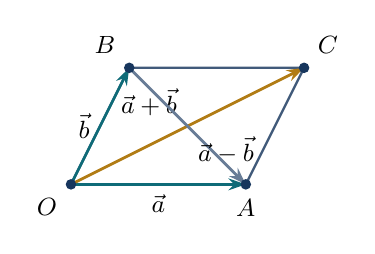
\begin{tikzpicture}[scale=.74,every node/.style={font=\small}]
  \coordinate (O) at (0,0); \coordinate (A) at (3,0); \coordinate (B) at (1,2); \coordinate (C) at (4,2);
  \draw[geom] (O)--(A)--(C)--(B)--cycle;
  \draw[vline] (O)--(A) node[midway,below] {$\vec a$}; \draw[vline] (O)--(B) node[midway,left] {$\vec b$};
  \draw[vline,draw=gold!90!black] (O)--(C) node[midway,above left] {$\vec a+\vec b$};
  \draw[vline,draw=navy!65] (B)--(A) node[midway,below right] {$\vec a-\vec b$};
  \node[vpoint,label=below left:$O$] at (O){}; \node[vpoint,label=below:$A$] at (A){}; \node[vpoint,label=above left:$B$] at (B){}; \node[vpoint,label=above right:$C$] at (C){};
\end{tikzpicture}}

\newcommand{\figBenz}{%
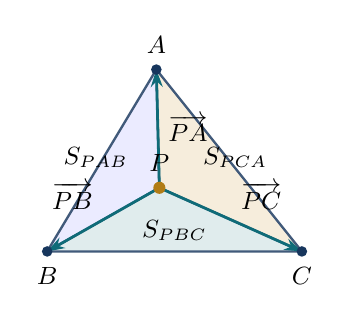
\begin{tikzpicture}[scale=.77,every node/.style={font=\small}]
  \coordinate (A) at (1.8,3.0); \coordinate (B) at (0,0); \coordinate (C) at (4.2,0); \coordinate (P) at (1.85,1.05);
  \fill[regionA] (P)--(B)--(C)--cycle; \fill[regionB] (P)--(C)--(A)--cycle; \fill[regionC] (P)--(A)--(B)--cycle;
  \draw[geom] (A)--(B)--(C)--cycle; \draw[geom] (P)--(A) (P)--(B) (P)--(C);
  \draw[vline] (P)--(A) node[midway,right] {$\overrightarrow{PA}$};
  \draw[vline] (P)--(B) node[midway,above left] {$\overrightarrow{PB}$};
  \draw[vline] (P)--(C) node[midway,above right] {$\overrightarrow{PC}$};
  \node[vpoint,label=above:$A$] at (A){}; \node[vpoint,label=below:$B$] at (B){}; \node[vpoint,label=below:$C$] at (C){}; \node[moving,label=above:$P$] at (P){};
  \node at (2.1,.35) {$S_{PBC}$}; \node at (3.1,1.55) {$S_{PCA}$}; \node at (.8,1.55) {$S_{PAB}$};
\end{tikzpicture}}

\newcommand{\figDotProduct}{%
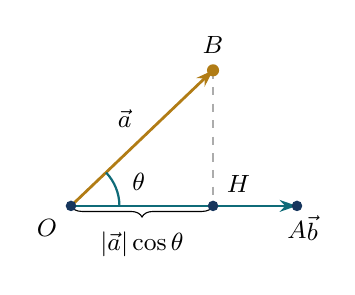
\begin{tikzpicture}[scale=.82,every node/.style={font=\small}]
  \coordinate (O) at (0,0); \coordinate (A) at (3.5,0); \coordinate (B) at (2.2,2.1); \coordinate (H) at (2.2,0);
  \draw[vline] (O)--(A); \node[below right] at (A) {$\vec b$};
  \draw[vline,draw=gold!90!black] (O)--(B) node[midway,above left] {$\vec a$};
  \draw[aid] (B)--(H);
  \draw[thick,teal] (0.75,0) arc[start angle=0,end angle=43.6,radius=.75];
  \node at (1.05,.38) {$\theta$};
  \draw[decorate,decoration={brace,amplitude=4pt,mirror}] (O)--(H) node[midway,below=6pt] {$|\vec a|\cos\theta$};
  \node[vpoint,label=below left:$O$] at (O){}; \node[vpoint,label=below:$A$] at (A){}; \node[moving,label=above:$B$] at (B){}; \node[vpoint,label=above right:$H$] at (H){};
\end{tikzpicture}}

\newcommand{\figPolarization}{%
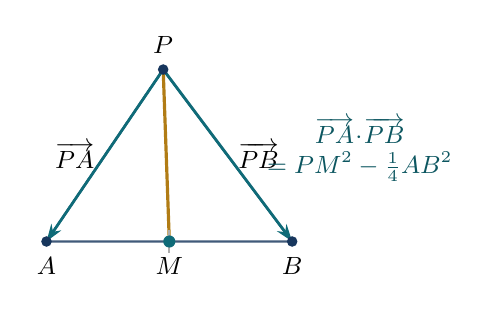
\begin{tikzpicture}[scale=.78,every node/.style={font=\small}]
  \coordinate (P) at (1.9,2.8); \coordinate (A) at (0,0); \coordinate (B) at (4,0); \coordinate (M) at (2,0);
  \draw[geom] (P)--(A)--(B)--cycle; \draw[hline] (P)--(M); \draw[aid] (M)+(0,.18)--+(0,-.18);
  \draw[vline] (P)--(A) node[midway,left] {$\overrightarrow{PA}$};
  \draw[vline] (P)--(B) node[midway,right] {$\overrightarrow{PB}$};
  \node[vpoint,label=above:$P$] at (P){}; \node[vpoint,label=below:$A$] at (A){}; \node[vpoint,label=below:$B$] at (B){}; \node[centerpt,label=below:$M$] at (M){};
  \node[align=center,text=teal!80!black] at (5.1,1.5) {$\overrightarrow{PA}\!\cdot\!\overrightarrow{PB}$\\$=PM^2-\frac14AB^2$};
\end{tikzpicture}}

\newcommand{\figCircleDistance}{%
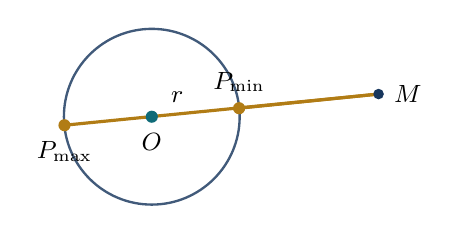
\begin{tikzpicture}[scale=.72,every node/.style={font=\small}]
  \coordinate (O) at (0,0); \coordinate (M) at (4.0,.4);
  \draw[geom] (O) circle (1.55);
  \coordinate (Pn) at (1.54,.15); \coordinate (Pf) at (-1.54,-.15);
  \draw[aid] (O)--(M); \draw[hline] (Pn)--(M); \draw[hline] (Pf)--(M);
  \node[centerpt,label=below:$O$] at (O){}; \node[vpoint,label=right:$M$] at (M){};
  \node[moving,label=above:$P_{\min}$] at (Pn){}; \node[moving,label=below:$P_{\max}$] at (Pf){};
  \node at (.45,.35) {$r$};
\end{tikzpicture}}

\newcommand{\figVectorCircle}{%
\begin{tikzpicture}[scale=.72,every node/.style={font=\small}]
  \coordinate (A) at (-2,0); \coordinate (B) at (2,0); \coordinate (M) at (0,0); \coordinate (X) at (1.1,1.65);
  \draw[geom] (M) circle (1.9); \draw[geom] (A)--(B); \draw[hline] (M)--(X);
  \draw[vline] (X)--(A); \draw[vline] (X)--(B);
  \node[vpoint,label=below:$A$] at (A){}; \node[vpoint,label=below:$B$] at (B){}; \node[centerpt,label=below:$M$] at (M){}; \node[moving,label=above:$X$] at (X){};
  \node[align=center] at (4.1,.7) {$XM^2=\frac14AB^2+k$\\轨迹为圆};
\end{tikzpicture}}

\newcommand{\figFourCenters}{%
\begin{tikzpicture}[scale=.75,every node/.style={font=\small}]
  \coordinate (A) at (1.6,3.0); \coordinate (B) at (0,0); \coordinate (C) at (4.3,0);
  \draw[geom] (A)--(B)--(C)--cycle;
  \coordinate (G) at (1.97,1.0); \coordinate (I) at (1.67,.88); \coordinate (O) at (2.15,.72); \coordinate (H) at (1.6,1.35);
  \node[centerpt,label=right:$G$] at (G){}; \node[moving,label=left:$I$] at (I){}; \node[vpoint,label=below:$O$] at (O){}; \node[vpoint,label=above:$H$] at (H){};
  \node[vpoint,label=above:$A$] at (A){}; \node[vpoint,label=below:$B$] at (B){}; \node[vpoint,label=below:$C$] at (C){};
  \node[align=left,text=gray!85!black] at (5.5,1.45) {重心 $G$：平均\\外心 $O$：等距\\内心 $I$：等角\\垂心 $H$：高线};
\end{tikzpicture}}

\newcommand{\figCentroid}{%
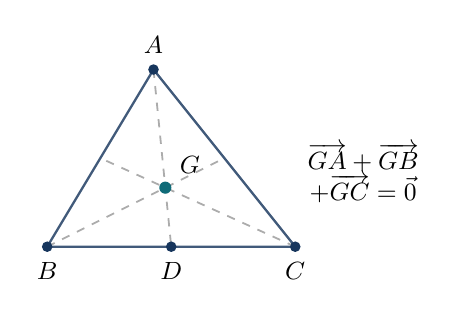
\begin{tikzpicture}[scale=.75,every node/.style={font=\small}]
  \coordinate (A) at (1.8,3); \coordinate (B) at (0,0); \coordinate (C) at (4.2,0);
  \coordinate (D) at ($(B)!.5!(C)$); \coordinate (E) at ($(C)!.5!(A)$); \coordinate (F) at ($(A)!.5!(B)$); \coordinate (G) at (2,1);
  \draw[geom] (A)--(B)--(C)--cycle; \draw[aid] (A)--(D) (B)--(E) (C)--(F);
  \node[centerpt,label=above right:$G$] at (G){}; \node[vpoint,label=above:$A$] at (A){}; \node[vpoint,label=below:$B$] at (B){}; \node[vpoint,label=below:$C$] at (C){};
  \node[vpoint,label=below:$D$] at (D){};
  \node[align=center] at (5.35,1.25) {$\overrightarrow{GA}+\overrightarrow{GB}$\\$+\overrightarrow{GC}=\vec0$};
\end{tikzpicture}}

\newcommand{\figCircumcenter}{%
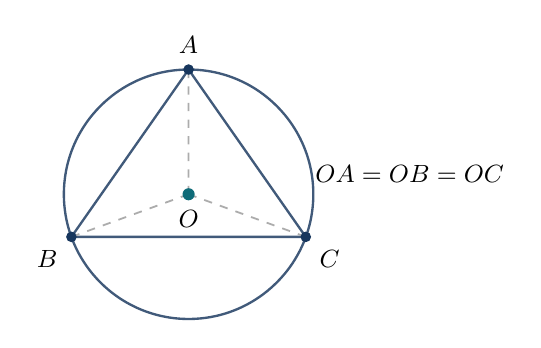
\begin{tikzpicture}[scale=.72,every node/.style={font=\small}]
  \coordinate (O) at (0,0); \coordinate (A) at (0,2.2); \coordinate (B) at (-2.067,-.752); \coordinate (C) at (2.067,-.752);
  \draw[geom] (O) circle (2.2); \draw[geom] (A)--(B)--(C)--cycle;
  \draw[aid] (O)--(A) (O)--(B) (O)--(C);
  \node[centerpt,label=below:$O$] at (O){}; \node[vpoint,label=above:$A$] at (A){}; \node[vpoint,label=below left:$B$] at (B){}; \node[vpoint,label=below right:$C$] at (C){};
  \node at (3.9,.35) {$OA=OB=OC$};
\end{tikzpicture}}

\newcommand{\figIncenter}{%
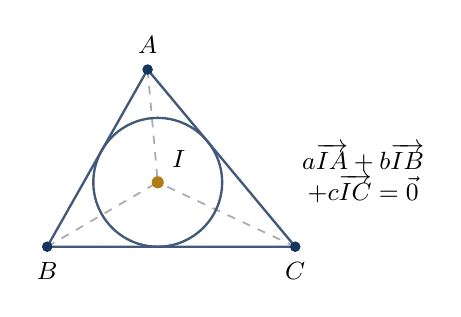
\begin{tikzpicture}[scale=.75,every node/.style={font=\small}]
  \coordinate (A) at (1.7,3); \coordinate (B) at (0,0); \coordinate (C) at (4.2,0); \coordinate (I) at (1.8715,1.0906);
  \draw[geom] (A)--(B)--(C)--cycle; \draw[aid] (A)--(I) (B)--(I) (C)--(I); \draw[geom] (I) circle (1.0906);
  \node[moving,label=above right:$I$] at (I){}; \node[vpoint,label=above:$A$] at (A){}; \node[vpoint,label=below:$B$] at (B){}; \node[vpoint,label=below:$C$] at (C){};
  \node[align=center] at (5.35,1.25) {$a\overrightarrow{IA}+b\overrightarrow{IB}$\\$+c\overrightarrow{IC}=\vec0$};
\end{tikzpicture}}

\newcommand{\figOrthocenter}{%
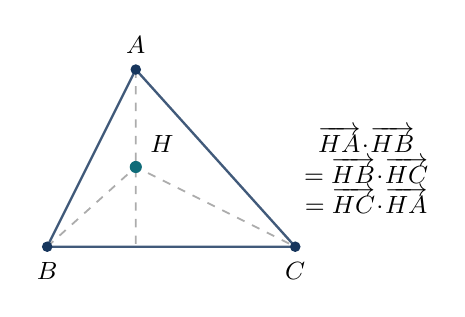
\begin{tikzpicture}[scale=.75,every node/.style={font=\small}]
  \coordinate (A) at (1.5,3); \coordinate (B) at (0,0); \coordinate (C) at (4.2,0); \coordinate (H) at (1.5,1.35);
  \draw[geom] (A)--(B)--(C)--cycle; \draw[aid] (A)--(1.5,0); \draw[aid] (B)--(H)--(C);
  \node[vpoint,label=above:$A$] at (A){}; \node[vpoint,label=below:$B$] at (B){}; \node[vpoint,label=below:$C$] at (C){}; \node[centerpt,label=above right:$H$] at (H){};
  \node[align=center] at (5.4,1.3) {$\overrightarrow{HA}\!\cdot\!\overrightarrow{HB}$\\$=\overrightarrow{HB}\!\cdot\!\overrightarrow{HC}$\\$=\overrightarrow{HC}\!\cdot\!\overrightarrow{HA}$};
\end{tikzpicture}}

\newcommand{\figEuler}{%
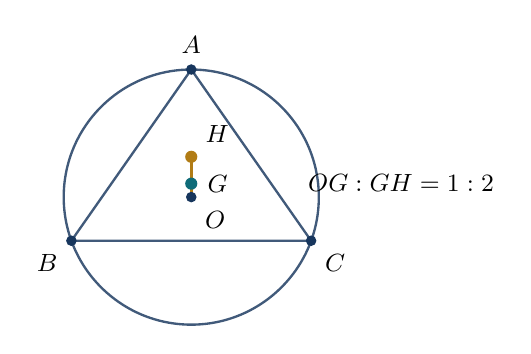
\begin{tikzpicture}[scale=.72,every node/.style={font=\small}]
  \coordinate (O) at (0,0); \coordinate (A) at (0,2.25); \coordinate (B) at (-2.114,-.77); \coordinate (C) at (2.114,-.77);
  \coordinate (G) at (0,.237); \coordinate (H) at (0,.711);
  \draw[geom] (O) circle (2.25); \draw[geom] (A)--(B)--(C)--cycle; \draw[hline] (O)--(H);
  \node[vpoint,label=below right:$O$] at (O){}; \node[centerpt,label=right:$G$] at (G){}; \node[moving,label=above right:$H$] at (H){};
  \node[vpoint,label=above:$A$] at (A){}; \node[vpoint,label=below left:$B$] at (B){}; \node[vpoint,label=below right:$C$] at (C){};
  \node at (3.7,.25) {$OG:GH=1:2$};
\end{tikzpicture}}


\newcommand{\figCentroidAverage}{%
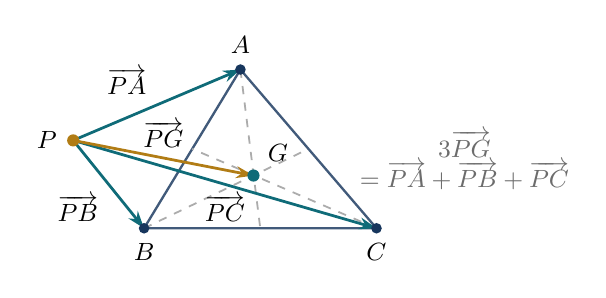
\begin{tikzpicture}[scale=.72,every node/.style={font=\small}]
  \coordinate (A) at (1.7,2.8); \coordinate (B) at (0,0); \coordinate (C) at (4.1,0);
  \coordinate (G) at (1.93,.93); \coordinate (P) at (-1.25,1.55);
  \draw[geom] (A)--(B)--(C)--cycle;
  \draw[aid] (A)--($(B)!.5!(C)$) (B)--($(A)!.5!(C)$) (C)--($(A)!.5!(B)$);
  \draw[vline] (P)--(A) node[midway,above left] {$\overrightarrow{PA}$};
  \draw[vline] (P)--(B) node[midway,below left] {$\overrightarrow{PB}$};
  \draw[vline] (P)--(C) node[midway,below] {$\overrightarrow{PC}$};
  \draw[vline,draw=gold!90!black] (P)--(G) node[midway,above] {$\overrightarrow{PG}$};
  \node[vpoint,label=above:$A$] at (A){}; \node[vpoint,label=below:$B$] at (B){};
  \node[vpoint,label=below:$C$] at (C){}; \node[centerpt,label=above right:$G$] at (G){};
  \node[moving,label=left:$P$] at (P){};
  \node[align=center,text=gray!85!black] at (5.65,1.2) {$3\overrightarrow{PG}$\\$=\overrightarrow{PA}+\overrightarrow{PB}+\overrightarrow{PC}$};
\end{tikzpicture}}

\newcommand{\figCircumProjection}{%
\begin{tikzpicture}[scale=.75,every node/.style={font=\small}]
  \coordinate (A) at (-2.2,0); \coordinate (B) at (2.2,0); \coordinate (M) at (0,0); \coordinate (O) at (0,2.35);
  \draw[geom] (A)--(B); \draw[aid] (O)--(M);
  \draw[vline] (A)--(B); \node[below right] at (1.0, 0) {$\overrightarrow{AB}$};
  \draw[vline,draw=gold!90!black] (A)--(O) node[midway,above left] {$\overrightarrow{AO}$};
  \draw pic[draw=teal,angle radius=5mm] {right angle=O--M--B};
  \node[vpoint,label=below left:$A$] at (A){}; \node[vpoint,label=below right:$B$] at (B){};
  \node[vpoint,label=above right:$M$] at (M){}; \node[centerpt,label=above:$O$] at (O){};
  \draw[decorate,decoration={brace,amplitude=4pt,mirror}] (A)--(M) node[midway,below=7pt] {$AB/2$};
  \node[align=left,text=gray!85!black] at (4.3,1.25) {沿 $AB$ 的数量投影\\恰为 $AM=AB/2$};
\end{tikzpicture}}

\newcommand{\figUnitBisectors}{%
\begin{tikzpicture}[scale=.72,every node/.style={font=\small}]
  \coordinate (A) at (0,0); \coordinate (U) at (2.4,0); \coordinate (V) at (1.2,2.078);
  \coordinate (S) at (3.6,2.078); \coordinate (D) at (1.2,-2.078);
  \draw[vline] (A)--(U) node[midway,below] {$\vec e_1$};
  \draw[vline] (A)--(V) node[midway,left] {$\vec e_2$};
  \draw[aid] (U)--(S)--(V);
  \draw[vline,draw=gold!90!black] (A)--(S) node[midway,above left] {$\vec e_1+\vec e_2$};
  \draw[vline,draw=navy!70] (A)--(D) node[midway,right] {$\vec e_1-\vec e_2$};
  \node[vpoint,label=below left:$A$] at (A){};
  \node[font=\footnotesize] at (1.2,-.28) {$1$}; \node[font=\footnotesize] at (.38,1.15) {$1$};
  \node[align=left,text=gray!85!black] at (5.15,.45) {和：内角平分线\\差：外角平分线};
\end{tikzpicture}}

\newcommand{\figRectangleObjective}{%
\begin{tikzpicture}[scale=.72,every node/.style={font=\small}]
  \coordinate (A) at (0,0); \coordinate (B) at (2.0,0); \coordinate (D) at (0,3.464); \coordinate (C) at (2.0,3.464);
  \coordinate (D0) at (0,1.155); \coordinate (P) at (1.225,1.225);
  \draw[geom] (A)--(B)--(C)--(D)--cycle; \draw[aid] (A) circle (1.732);
  \draw[aid] (-0.5,1.655)--(2.2,-0.5) node[right,font=\scriptsize,text=gray!70!black] {等和基线 \(\lambda+\sqrt3\mu=1\)};
  \draw[hline] (-0.2,2.65)--(2.65,-0.2) node[right,font=\scriptsize,text=gold!90!black] {等和切线 \(\lambda+\sqrt3\mu=\frac{\sqrt6}{2}\)};
  \draw[vline,draw=gold!90!black] (A)--(P); \draw[aid,draw=teal] (A)--(P);
  \node[vpoint,label=below left:$A$] at (A){}; \node[vpoint,label=below:$B$] at (B){}; \node[vpoint,label=above:$C$] at (C){}; \node[vpoint,label=left:$D$] at (D){};
  \node[moving,label=above right:$P$] at (P){}; \node[vpoint,label=left:$D_0$] at (D0){};
\end{tikzpicture}}

\newcommand{\figEquilateralDiameter}{%
\begin{tikzpicture}[scale=.78,every node/.style={font=\small}]
  \coordinate (B) at (-2,0); \coordinate (C) at (2,0); \coordinate (A) at (0,3.464); \coordinate (O) at (0,0);
  \coordinate (C0) at (1,1.732); \coordinate (P) at (1,-1.732);
  \draw[geom] (O) circle (2);
  \draw[geom] (A)--(B)--(C)--cycle;
  \draw[aid] (-2.5,-0.288)--(1.6,2.078) node[right,font=\scriptsize,text=gray!70!black] {等和基线 \(\lambda+2\mu=1\)};
  \draw[hline] (-0.8,-2.771)--(2.8,-0.693) node[right,font=\scriptsize,text=gold!90!black] {等和切线 \(\lambda+2\mu=\frac{5}{2}\)};
  \draw[vline,draw=gold!90!black] (A)--(P);
  \draw[aid,draw=teal] (O)--(P);
  \node[vpoint,label=above:$A$] at (A){}; \node[vpoint,label=left:$B$] at (B){}; \node[vpoint,label=right:$C$] at (C){};
  \node[moving,label=below right:$P$] at (P){}; \node[centerpt,label=above left:$O$] at (O){};
  \node[vpoint,label=right:$C_0$] at (C0){};
\end{tikzpicture}}

\newcommand{\figHexagonDisk}{%
\begin{tikzpicture}[scale=.64,every node/.style={font=\small}]
  \coordinate (A) at (90:2.3); \coordinate (B) at (30:2.3); \coordinate (C) at (-30:2.3);
  \coordinate (D) at (-90:2.3); \coordinate (E) at (-150:2.3); \coordinate (F) at (150:2.3);
  \draw[geom] (A)--(B)--(C)--(D)--(E)--(F)--cycle;
  \draw[aid] ($(B)+(-0.5,0.866)$)--($(F)+(0.5,-0.866)$) node[left,font=\scriptsize,text=gray!70!black] {等和基线 \(m+n=1\)};
  \coordinate (Q) at (D); \draw[geom,fill=teal!8] (Q) circle (1.15);
  \coordinate (P) at ($(D)+(270:1.15)$);
  \draw[hline] ($(D)+(-1.5,0)$)--($(D)+(1.5,0)$) node[right,font=\scriptsize,text=gold!90!black] {等和切线 \(m+n=5\)};
  \draw[vline,draw=gold!90!black] (A)--(P);
  \node[centerpt,label=above left:$Q$] at (Q){}; \node[moving,label=below:$P$] at (P){};
  \node[vpoint,label=above:$A$] at (A){}; \node[vpoint,label=above right:$B$] at (B){};
  \node[vpoint,label=below right:$C$] at (C){}; \node[vpoint,label=right:$D$] at (D){};
  \node[vpoint,label=below left:$E$] at (E){}; \node[vpoint,label=above left:$F$] at (F){};
\end{tikzpicture}}

\newcommand{\figSquareDisk}{%
\begin{tikzpicture}[scale=.64,every node/.style={font=\small}]
  \coordinate (A) at (0,3.6); \coordinate (B) at (0,0); \coordinate (C) at (3.6,0); \coordinate (D) at (3.6,3.6);
  \draw[geom] (A)--(B)--(C)--(D)--cycle;
  \draw[aid] (-0.8,4.4)--(4.4,-0.8) node[right,font=\scriptsize,text=gray!70!black] {等和基线 \(m+n=1\)};
  \coordinate (Q1) at (C); \draw[geom,fill=teal!8] (Q1) circle (0.9); \coordinate (P1) at ($(C)+(-135:0.9)$);
  \draw[hline] (-1.2,2.5)--(2.5,-1.2) node[below left,font=\scriptsize,text=gold!90!black] {下切线 \(m+n=1-\frac{\sqrt2}{4}\)};
  \coordinate (Q2) at (D); \draw[geom,fill=teal!8] (Q2) circle (0.9); \coordinate (P2) at ($(D)+(45:0.9)$);
  \draw[hline] (1.2,6.0)--(6.0,1.2) node[above right,font=\scriptsize,text=gold!90!black] {上切线 \(m+n=2+\frac{\sqrt2}{4}\)};
  \node[vpoint,label=above left:$A$] at (A){}; \node[vpoint,label=below left:$B$] at (B){}; \node[vpoint,label=below:$C$] at (C){}; \node[vpoint,label=above:$D$] at (D){};
  \node[moving,label=below left:$P_1$] at (P1){}; \node[moving,label=above right:$P_2$] at (P2){};
\end{tikzpicture}}

\newcommand{\figTwoCircles}{%
\begin{tikzpicture}[scale=.68,every node/.style={font=\small}]
  \coordinate (O) at (0,0); \coordinate (A) at (0,2.45); \coordinate (B) at (-2.122,-1.225); \coordinate (C) at (2.122,-1.225);
  \draw[geom] (O) circle (2.45); \draw[geom] (O) circle (1.225); \draw[geom] (A)--(B)--(C)--cycle;
  \draw[aid] (-2.8,-1.225)--(2.8,-1.225) node[right,font=\scriptsize,text=gray!70!black] {基线 \(x+y=1\) (BC)};
  \coordinate (P) at (0,-2.45); \coordinate (Q) at (0,-1.225);
  \draw[hline] (-2.8,-2.45)--(2.8,-2.45) node[right,font=\scriptsize,text=gold!90!black] {外切线 \(x_1+y_1=\frac{4}{3}\)};
  \draw[hline] (-2.2,-1.225)--(2.2,-1.225);
  \node[moving,label=below:$P_{\max}$] at (P){}; \node[centerpt,label=above:$Q_{\min}$] at (Q){};
  \node[vpoint,label=above:$A$] at (A){}; \node[vpoint,label=below left:$B$] at (B){}; \node[vpoint,label=below right:$C$] at (C){}; \node[vpoint,label=above left:$O$] at (O){};
\end{tikzpicture}}

\newcommand{\figAngleBisector}{%
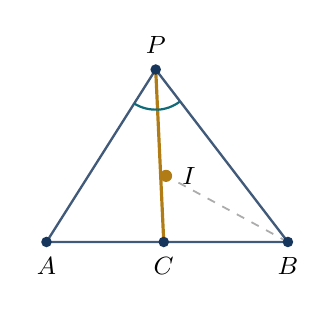
\begin{tikzpicture}[scale=.73,every node/.style={font=\small}]
  \coordinate (P) at (1.9,3); \coordinate (A) at (0,0); \coordinate (B) at (4.2,0); \coordinate (C) at (2.04,0); \coordinate (I) at (2.08,1.15);
  \draw[geom] (P)--(A)--(B)--cycle; \draw[hline] (P)--(C); \draw[aid] (B)--(I);
  \node[vpoint,label=above:$P$] at (P){}; \node[vpoint,label=below:$A$] at (A){}; \node[vpoint,label=below:$B$] at (B){}; \node[vpoint,label=below:$C$] at (C){}; \node[moving,label=right:$I$] at (I){};
  \draw[teal,thick] ($(P)!7mm!(A)$) arc[start angle=238,end angle=273,radius=7mm];
  \draw[teal,thick] ($(P)!7mm!(C)$) arc[start angle=273,end angle=307,radius=7mm];
\end{tikzpicture}}

\newcommand{\figIsoscelesOrthocenter}{%
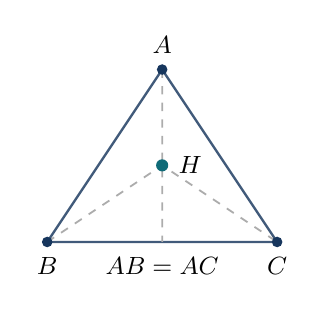
\begin{tikzpicture}[scale=.73,every node/.style={font=\small}]
  \coordinate (A) at (2,3); \coordinate (B) at (0,0); \coordinate (C) at (4,0); \coordinate (H) at (2,1.333);
  \draw[geom] (A)--(B)--(C)--cycle; \draw[aid] (A)--(2,0); \draw[aid] (B)--(H)--(C);
  \node[vpoint,label=above:$A$] at (A){}; \node[vpoint,label=below:$B$] at (B){}; \node[vpoint,label=below:$C$] at (C){}; \node[centerpt,label=right:$H$] at (H){};
  \node at (2,-.42) {$AB=AC$};
\end{tikzpicture}}

\newcommand{\figMovingMidpoint}{%
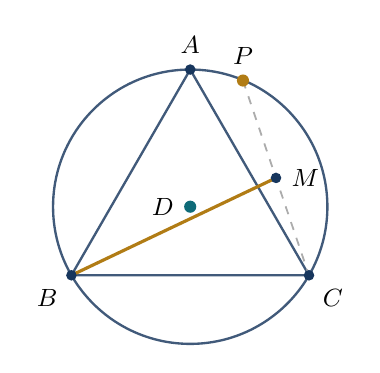
\begin{tikzpicture}[scale=.67,every node/.style={font=\small}]
  \coordinate (D) at (0,0); \coordinate (A) at (0,2.6); \coordinate (B) at (-2.2517,-1.3); \coordinate (C) at (2.2517,-1.3); \coordinate (P) at (1.0,2.3916); \coordinate (M) at ($(P)!.5!(C)$);
  \draw[geom] (D) circle (2.6); \draw[geom] (A)--(B)--(C)--cycle; \draw[aid] (P)--(C); \draw[hline] (B)--(M);
  \node[centerpt,label=left:$D$] at (D){}; \node[vpoint,label=above:$A$] at (A){}; \node[vpoint,label=below left:$B$] at (B){}; \node[vpoint,label=below right:$C$] at (C){}; \node[moving,label=above:$P$] at (P){}; \node[vpoint,label=right:$M$] at (M){};
\end{tikzpicture}}

\begin{document}
\frontmatter
\begin{titlepage}
\centering
\vspace*{2.2cm}
{\Huge\bfseries\sffamily\color{navy} 高中数学·平面向量}\par
\vspace{0.5cm}
{\LARGE\bfseries\sffamily\color{teal}图解教案与完整题型讲义}\par
\vspace{0.8cm}
{\large 线性组合—等和线—数量积—极化恒等式—三角形四心}\par
\vfill
\begin{tcolorbox}[width=.82\textwidth,colback=bluegray,colframe=navy,arc=3mm]
\centering
\textbf{编写说明}\par
本讲义以“位置关系用线性组合，度量关系用数量积，动点问题用轨迹转化”为主线，\par
吸收《等和线》《向量四心大总结》中的典型题型，并补足基础概念、\par
平面向量基本定理、坐标法、数量积、极化恒等式、面积坐标与奔驰定理等内容。
\end{tcolorbox}
\vfill
{\large 教师用·图解授课·可直接二次改编}\par
\vspace*{1.5cm}
\end{titlepage}

\chapter*{使用说明与课程总览}
\addcontentsline{toc}{chapter}{使用说明与课程总览}

\begin{teachbox}
\textbf{建议课时：}基础班 14--16 课时，培优班 18--22 课时。每章按照“核心问题—图形建构—例题解析—方法提炼—易错诊断”组织。所有示意图均服务于推理，不按比例绘制。

\textbf{三条总主线：}
\begin{enumerate}
  \item \textbf{线性组合主线：}加减、数乘、基底、分点、共线、等和线、面积坐标；
  \item \textbf{数量积主线：}长度、夹角、垂直、投影、平方化、极化恒等式；
  \item \textbf{轨迹转化主线：}直线族、圆、线段、圆弧、中点轨迹、距离最值与取值范围。
\end{enumerate}
\end{teachbox}

\begin{methodbox}[title={图示阅读规则}]
图中的蓝色线表示原图结构，青色箭头表示向量或关键方向，金色线表示当前解题中真正使用的轨迹、截线或中线。学生应先读图，再写出对应的向量关系；不要从示意图目测长度、角度或比例。
\end{methodbox}

\begin{center}
\begin{tabularx}{0.96\textwidth}{>{\bfseries}c X X}
\toprule
课次 & 主讲内容 & 建议课堂产出\\
\midrule
1--2 & 向量语言、加减与数乘 & 会统一起点、检查箭头方向\\
3--4 & 基底、分点、共线与等和线 & 会把点的位置写成系数组合\\
5--6 & 等和线的截距模型、参数最值 & 会从系数约束识别轨迹\\
7--8 & 坐标与数量积 & 会把长度、角度、垂直数字化\\
9 & 极化恒等式 & 会把点积转化为到中点的距离\\
10 & 面积坐标与奔驰定理 & 会在面积比与向量系数间转换\\
11--12 & 四心的统一向量刻画 & 会从“等距、等点积、向量和”识别中心\\
13--16 & 四心进阶与综合 & 会选择基底法、坐标法、数量积法\\
\bottomrule
\end{tabularx}
\end{center}

\tableofcontents

\mainmatter
\part{基础语言与线性结构}

\chapter{向量的概念、表示与线性运算}

\begin{teachbox}
\textbf{本章必须讲透：}向量与线段的区别；箭头方向；自由向量；零向量的边界；同起点相减的方向。

\textbf{适合学生自行推导：}三角形法则、多边形法则、平行四边形法则之间的统一。
\end{teachbox}

\section{向量是什么}
向量由\textbf{大小}和\textbf{方向}共同确定。几何上用有向线段表示：
\[
\vect{AB},\qquad |\vect{AB}|=AB.
\]
向量是自由向量，只要大小相等、方向相同，即使起点不同，也表示同一个向量。
\figcap{\figVectorLanguage}{相等向量只比较大小和方向；相反向量方向相反且模相等。}

\begin{warningbox}
\[
\vect{AB}=-\vect{BA},\qquad AB=BA.
\]
左边是向量，右边是线段长度。零向量没有确定方向；讨论夹角时通常要求两个向量均非零。
\end{warningbox}

\section{加法、减法和数乘}
\begin{theorembox}{三角形法则与多边形法则}
\[
\vect{AB}+\vect{BC}=\vect{AC},
\]
进一步有
\[
\vect{A_1A_2}+\vect{A_2A_3}+\cdots+\vect{A_{n-1}A_n}=\vect{A_1A_n}.
\]
\end{theorembox}
\figcap{\figVectorAdd}{首尾相接的两段位移，等价于从起点直接指向终点的位移。}

同起点向量相减时：
\[
\vect{OA}-\vect{OB}=\vect{BA}.
\]
可以用一句话检查方向：\textbf{从减数的终点指向被减数的终点}。

数乘满足
\[
|\lambda\vv a|=|\lambda|\,|\vv a|.
\]
当 \(\lambda>0\) 时同向，\(\lambda<0\) 时反向，\(\lambda=0\) 时得到零向量。

\begin{problem}{向量式化简：先统一起点}
化简
\[
\vect{AB}+\vect{DC}-\vect{AC}-\vect{DB}.
\]
\end{problem}
\begin{solution}
\figcap{\figVectorAdd}{把首尾相接和同起点相减统一到同一幅图中。}
把所有向量用位置向量表示：
\[
(B-A)+(C-D)-(C-A)-(B-D)=\vv0.
\]
也可以先组合 \(\vect{AB}-\vect{AC}=\vect{CB}\)，再与 \(\vect{DC}-\vect{DB}=\vect{BC}\) 相加。
\ans{\vv0}
\end{solution}

\begin{problem}{数乘的方向与零向量边界}
已知非零向量 \(\vv a\)，判断 \(-3\vv a\)、\(\tfrac12\vv a\)、\(\vv0\) 与 \(\vv a\) 的方向关系。
\end{problem}
\begin{solution}
\figcap{\figVectorLanguage}{正倍数同向，负倍数反向；零向量只讨论平行，不讨论确定方向。}
\(-3\vv a\) 与 \(\vv a\) 反向；\(\tfrac12\vv a\) 与 \(\vv a\) 同向；零向量没有确定方向，但按高中教材约定，零向量与任意向量平行。
\end{solution}

\begin{summarybox}{本章一句话}
向量加减描述“位移如何合成”，数乘描述“沿同一方向伸缩或反向”。后续所有复杂式子，第一步都应先统一起点和方向。
\end{summarybox}

\chapter{平面向量基本定理、分点与共线}

\begin{teachbox}
\textbf{核心问题：}为什么两个不共线方向能控制整个平面？为什么能够比较系数？

\textbf{板书主线：}线性组合 \(\to\) 基底唯一性 \(\to\) 分点公式 \(\to\) 三点共线。
\end{teachbox}

\section{平面向量基本定理}
\begin{theorembox}{平面向量基本定理}
若 \(\vv e_1,\vv e_2\) 不共线，则平面内任意向量 \(\vv p\) 都存在唯一实数 \(x,y\)，使
\[
\vv p=x\vv e_1+y\vv e_2.
\]
\end{theorembox}
\figcap{\figBasis}{两个不共线方向提供两个自由度；虚线平行四边形展示线性组合。}
“存在”说明两个方向能张成整个平面；“唯一”说明同一基底下可以比较系数：
\[
x_1\vv e_1+y_1\vv e_2=x_2\vv e_1+y_2\vv e_2
\Longrightarrow x_1=x_2,\ y_1=y_2.
\]

\section{分点公式与仿射组合}
若 \(P\) 在直线 \(BC\) 上，且
\[
\vect{BP}=t\vect{BC},
\]
则
\[
\boxed{\vect{AP}=(1-t)\vect{AB}+t\vect{AC}}.
\]
特别地，若 \(BP:PC=m:n\)，则
\[
\boxed{\vect{AP}=\frac{n}{m+n}\vect{AB}+\frac{m}{m+n}\vect{AC}}.
\]
系数之所以“交叉”，来自 \(t=BP/BC=m/(m+n)\)。
\figcap{\figDivision}{点 P 在线段 BC 上时，位置向量是端点位置的加权平均。}

\begin{theorembox}{三点共线的系数判定}
若 \(\vect{AB},\vect{AC}\) 不共线，且
\[
\vect{AP}=\lambda\vect{AB}+\mu\vect{AC},
\]
则
\[
B,P,C\text{ 共线}\Longleftrightarrow \lambda+\mu=1.
\]
若还要求 \(P\) 在线段 \(BC\) 内，则需进一步满足 \(\lambda,\mu\ge0\)。
\end{theorembox}
\figcap{\figEqualSum}{系数和为 1 得到直线 BC；系数和为常数 k 得到与 BC 平行的直线。}

\begin{problem}{分点系数与三点共线}
在 \(\triangle ABC\) 中，点 \(D\) 在 \(AC\) 上，且
\[
\vect{AD}=\frac13\vect{DC}.
\]
点 \(P\) 在线段 \(BD\) 上，若
\[
\vect{AP}=m\vect{AB}+\frac16\vect{AC},
\]
求 \(m\)。
\end{problem}
\begin{solution}
\figcap{\figDP}{D 将 AC 按 1:3 分割，P 位于 BD 上；图中没有额外辅助点。}
由 \(AD:DC=1:3\)，得 \(AC=4AD\)，故
\[
\frac16\vect{AC}=\frac23\vect{AD}.
\]
于是
\[
\vect{AP}=m\vect{AB}+\frac23\vect{AD}.
\]
因为 \(B,P,D\) 共线，以 \(\vect{AB},\vect{AD}\) 为基底时两系数和为 \(1\)，所以
\[
m+\frac23=1.
\]
\ans{m=\frac13}
\end{solution}

\begin{problem}{过重心的截线与系数和}
点 \(O\) 是 \(\triangle ABC\) 的重心。过 \(O\) 的直线分别交 \(AB,AC\) 于 \(M,N\)，\(D\) 为 \(BC\) 中点。若
\[
\vect{AD}=x\vect{AM}+y\vect{AN},
\]
求 \(x+y\)。
\end{problem}
\begin{solution}
\figcap{\figCentroidCross}{D 是 BC 中点，G 是重心，过 G 的截线交 AB、AC 于 M、N。}
重心在中线上满足
\[
\vect{AO}=\frac23\vect{AD},\qquad \vect{AD}=\frac32\vect{AO}.
\]
又因 \(M,O,N\) 共线，存在 \(\alpha+\beta=1\)，使
\[
\vect{AO}=\alpha\vect{AM}+\beta\vect{AN}.
\]
因此
\[
\vect{AD}=\frac32\alpha\vect{AM}+\frac32\beta\vect{AN},
\]
故 \(x+y=\frac32(\alpha+\beta)\)。
\ans{\frac32}
\end{solution}

\begin{problem}{共线约束下的倒数和最值}
在 \(\triangle ABC\) 中，点 \(D\) 在线段 \(AB\) 内，且
\[
\vect{CD}=x\vect{CA}+y\vect{CB}.
\]
求 \(\dfrac1x+\dfrac2y\) 的最小值。
\end{problem}
\begin{solution}
\figcap{\figDOnAB}{D 在线段 AB 内，向量 CD 由 CA、CB 的正系数组合表示。}
因为 \(A,D,B\) 共线且 \(D\) 在线段内部，故
\[
x+y=1,\qquad x>0,\ y>0.
\]
由柯西不等式
\[
\left(\frac1x+\frac2y\right)(x+y)\ge(1+\sqrt2)^2.
\]
代入 \(x+y=1\)，得
\ans{3+2\sqrt2}
等号在 \(x:y=1:\sqrt2\) 时成立。
\end{solution}

\begin{methodbox}
对正数 \(x,y\) 且 \(x+y=k\)，常用模板
\[
\min\left(\frac{a}{x}+\frac{b}{y}\right)=\frac{(\sqrt a+\sqrt b)^2}{k}.
\]
等和线题经常把几何关系压缩成这个代数模型。
\end{methodbox}

\begin{problem}{中线参数与截距关系}
在 \(\triangle ABC\) 中，\(O\) 为 \(BC\) 中点，\(\vect{AP}=t\vect{AO}\)。过 \(P\) 的直线分别交 \(AB,AC\) 于 \(M,N\)，且
\[
\vect{AM}=m\vect{AB},\qquad \vect{AN}=n\vect{AC}.
\]
求 \(\dfrac1m+\dfrac1n\)。
\end{problem}
\begin{solution}
\figcap{\figMedianCross}{O 是 BC 中点，P 在中线 AO 上；过 P 的直线以 M、N 为两个截距点。}
\[
\vect{AP}=t\vect{AO}=\frac t2\vect{AB}+\frac t2\vect{AC}.
\]
而 \(P\in MN\)，以截距向量 \(\vect{AM}=m\vect{AB}\)、\(\vect{AN}=n\vect{AC}\) 表示时，系数和为 \(1\)：
\[
\frac{t/2}{m}+\frac{t/2}{n}=1.
\]
\ans{\frac1m+\frac1n=\frac2t}
\end{solution}

\begin{summarybox}{本章一句话}
“系数和为 \(1\)”不是记忆技巧，而是点在线段（或直线）上的仿射表示；“同一向量两种表示”则依赖基底表示的唯一性。
\end{summarybox}

\chapter{等和线、截距模型与参数优化}

\begin{teachbox}
\textbf{教学重点：}把“系数和固定”看成一族平行线；把“过定点作截线”转化为倒数约束；处理端点、正负与能否取等。
\end{teachbox}

\section{等和线的一般形式}
若
\[
\vect{AP}=\lambda\vect{AB}+\mu\vect{AC},\qquad \lambda+\mu=k,
\]
则
\[
\vect{AP}=k\vect{AC}+\lambda\vect{CB}.
\]
取点 \(Q\) 使 \(\vect{AQ}=k\vect{AC}\)，则 \(\vect{QP}=\lambda\vect{CB}\)，故 \(P\) 的轨迹是一条过 \(Q\) 且平行于 \(BC\) 的直线。
\figcap{\figEqualSumGeneral}{改变参数只让点沿平行于 BC 的方向移动；改变系数和才会更换平行线。}

\begin{warningbox}
\(\lambda+\mu=1\) 只保证 \(P\) 在直线 \(BC\) 上，不保证在线段内。要在线段内还需 \(\lambda,\mu\ge0\)。
\end{warningbox}

\section{截距式：一条直线与两条基向量轴}
若点 \(P\) 在连接 \(M=m\vv a\) 与 \(N=n\vv b\) 的直线上，且
\[
\vect{OP}=\alpha\vv a+\beta\vv b,
\]
则
\[
\boxed{\frac{\alpha}{m}+\frac{\beta}{n}=1}.
\]
这就是向量形式的直线截距式。

\begin{problem}{两条劈线交点与截距最值}
在 \(\triangle ABC\) 中，\(D\) 为 \(AC\) 中点；点 \(E\in BC\) 满足 \(EC=3BE\)；\(P=BD\cap AE\)。过 \(P\) 作一直线，分别交 \(AC,BC\) 于 \(M,N\)。设
\[
\vect{CM}=m\vect{CA},\qquad \vect{CN}=n\vect{CB},
\]
求 \(m+n\) 的最小值。
\end{problem}
\begin{solution}
\figcap{\figComplexCevian}{D 是 AC 中点，E 将 BC 按 1:3 分割；P 是 BD 与 AE 的交点。}
以 \(C\) 为起点，取 \(\vect{CA},\vect{CB}\) 为基底。由
\[
\vect{CD}=\frac12\vect{CA},\qquad \vect{CE}=\frac34\vect{CB},
\]
联立直线 \(BD\) 与 \(AE\) 的参数式，可得
\[
\vect{CP}=\frac15\vect{CA}+\frac35\vect{CB}.
\]
因为 \(P\in MN\)，截距式给出
\[
\frac{1/5}{m}+\frac{3/5}{n}=1
\quad\Longleftrightarrow\quad
\frac1m+\frac3n=5.
\]
由柯西不等式
\[
(m+n)\left(\frac1m+\frac3n\right)\ge(1+\sqrt3)^2,
\]
故
\ans{\min(m+n)=\frac{4+2\sqrt3}{5}}
\end{solution}

\begin{problem}{缩放向量后的等和约束}
在 \(\triangle ABC\) 中，点 \(D\) 在 \(AB\) 上运动，且 \(D\ne A,B\)。点 \(E\) 满足
\[
\vect{CE}=\frac13\vect{CD},\qquad
\vect{CE}=\lambda\vect{CA}+\mu\vect{CB}.
\]
求 \(\dfrac3\lambda+\dfrac1\mu\) 的最小值。
\end{problem}
\begin{solution}
\figcap{\figScaledE}{D 在 AB 上运动，E 是线段 CD 上满足 CE=CD/3 的缩放点。}
因为 \(D\in AB\)，可写
\[
\vect{CD}=x\vect{CA}+y\vect{CB},\qquad x+y=1,
\]
且 \(x,y>0\)。因此
\[
\lambda=\frac x3,
\qquad \mu=\frac y3,
\qquad \lambda+\mu=\frac13.
\]
于是
\[
\left(\frac3\lambda+\frac1\mu\right)(\lambda+\mu)
\ge(\sqrt3+1)^2.
\]
\ans{12+6\sqrt3}
\end{solution}

\begin{problem}{两条劈线交点的基底表示}
在 \(\triangle ABC\) 中，\(D,E\) 分别满足
\[
\vect{AD}=\frac12\vect{AB},\qquad
\vect{AE}=\frac13\vect{AC},
\]
直线 \(CD\) 与 \(BE\) 交于 \(P\)。
\begin{enumerate}[label=(\arabic*)]
\item 用 \(\vect{AB},\vect{AC}\) 表示 \(\vect{AP}\)；
\item 过 \(P\) 的直线交射线 \(AB,AC\) 于 \(M,N\)，设 \(\vect{AM}=m\vect{AB}\)、\(\vect{AN}=n\vect{AC}\)，求 \(m+n\) 的最小值。
\end{enumerate}
\end{problem}
\begin{solution}
\figcap{\figTwoCevianExact}{D、E 分别是 AB、AC 上的定比分点，P 是 CD 与 BE 的交点。}
设
\[
\vect{AP}=x\vect{AB}+y\vect{AC}.
\]
由 \(P\in CD\) 与 \(P\in BE\) 分别写参数式并比较系数，得
\[
x=\frac25,
\qquad y=\frac15.
\]
故
\[
\boxed{\vect{AP}=\frac25\vect{AB}+\frac15\vect{AC}}.
\]
再由截距式
\[
\frac{2/5}{m}+\frac{1/5}{n}=1
\quad\Longleftrightarrow\quad
\frac2m+\frac1n=5.
\]
所以
\[
(m+n)\left(\frac2m+\frac1n\right)\ge(\sqrt2+1)^2,
\]
从而
\ans{\min(m+n)=\frac{3+2\sqrt2}{5}}
\end{solution}

\begin{problem}{系数比例、边长与面积最值}
在 \(\triangle ABC\) 中，点 \(D\in AB\) 且 \(AD=\frac13AB\)，\(E\) 是 \(CD\) 的中点，直线 \(AE\) 交 \(BC\) 于 \(H\)。点 \(P\) 在直线 \(AH\) 上运动，且
\[
\vect{AP}=\lambda\vect{AB}+\mu\vect{AC}.
\]
已知 \(AB=4\)，并满足 \(\lambda\,AC=\mu\,BC\)，求 \(\triangle CAH\) 面积的最大值。
\end{problem}
\begin{solution}
\figcap{\figAEH}{D 是 AB 的三分点，E 是 CD 中点，H 是 AE 与 BC 的交点，P 沿 AH 运动。}
以 \(A\) 为起点，令 \(\vect{AB}=\vv b,\vect{AC}=\vv c\)。由
\[
\vect{AD}=\frac13\vv b,
\qquad
\vect{AE}=\frac16\vv b+\frac12\vv c,
\]
可得直线 \(AE\) 与 \(BC\) 的交点满足
\[
\vect{AH}=\frac14\vv b+\frac34\vv c.
\]
因此直线 \(AH\) 上任一点的系数满足 \(\mu=3\lambda\)。由题设 \(\lambda AC=\mu BC\)，且 \(P\ne A\)，得到
\[
AC=3BC.
\]
设 \(BC=a\)，则 \(AC=3a,AB=4\)。又 \(BH:HC=3:1\)，故
\[
[CAH]=\frac14[ABC].
\]
由海伦公式或面积恒等式
\[
[ABC]^2=4(4-a^2)(a^2-1),\qquad 1<a<2.
\]
令 \(x=a^2\)，乘积 \((4-x)(x-1)\) 在 \(x=\frac52\) 时最大，故 \([ABC]_{\max}=3\)。
\ans{[CAH]_{\max}=\frac34}
\end{solution}

\begin{summarybox}{截距模型的统一流程}
先求定点 \(P\) 在所选基底下的系数 \((\alpha,\beta)\)，再对动截线写
\[
\frac{\alpha}{m}+\frac{\beta}{n}=1,
\]
最后用柯西、均值不等式或判别式处理 \(m+n\)、\(1/m+1/n\) 等目标。
\end{summarybox}

\chapter{线性函数、圆与多边形轨迹}

\begin{tcolorbox}[colback=teal!5,colframe=teal!80!black,arc=2mm,boxrule=0.9pt,title={\bfseries\sffamily\color{white} 解疑精讲：等和线的值到底怎么算？（图解三条法则与误区澄清）}]
\small
\textbf{【常见误区澄清】}
等和线的值 \(k\) \textbf{不等于} 原点到直线的垂线长度！垂线长度是几何距离（标量），而等和线的值 \(k\) 是向量在斜坐标系/特定基底下的\textbf{线性加权系数和}。

\vspace{0.4em}
\textbf{【法则一：截距比例法（几何最速法）】}
\begin{enumerate}
  \item 先画出 \(k=1\) 时的\textbf{等和基线 \(L_1\)}：\(a\lambda + b\mu = 1 \iff \frac{\lambda}{1/a} + \frac{\mu}{1/b} = 1\)，两轴截距为 \(B_0\left(\frac{1}{a}\vect{AB}\right)\) 与 \(C_0\left(\frac{1}{b}\vect{AC}\right)\)；
  \item 过切点 \(P\) 作 \(L_1\) 的平行切线/轨迹线 \(L_k\)，交两轴于 \(B_k, C_k\)；
  \item 则等和线的值 \(k\) 即为两截距的比值：\(k = \dfrac{AB_k}{AB_0} = \dfrac{AC_k}{AC_0}\)。
\end{enumerate}

\figcap{\figInterceptRatio}{法则一图解：等和线的值 \(k\) 即为平移平行线 \(L_k\) 在基底轴上的截距与基线 \(L_1\) 截距的比值。}

\vspace{0.4em}
\textbf{【法则二：直角坐标代换法（最可靠通法）】}
\begin{enumerate}
  \item 建系将 \(\vect{AP} = \lambda\vect{AB} + \mu\vect{AC}\) 转为直角坐标 \((x,y)\)，反解出 \(\lambda, \mu\)；
  \item 将 \(a\lambda + b\mu\) 化为直角坐标下的线性函数 \(Ax + By\)；
  \item 求出切点/极值点 \(P(x_0, y_0)\) 的坐标，\textbf{直接代入计算}：\(k = Ax_0 + By_0\)。
\end{enumerate}

\vspace{0.4em}
\textbf{【法则三：投影点积法（如何构造 \(\vec m\) 与数值代算流程）】}
\begin{enumerate}
  \item \textbf{第一步：如何精确构造辅助向量 \(\vec m\)}：
        设 \(\vec m = x \vect{AB} + y \vect{AC}\)，要求 \(\vect{AP} \cdot \vec m = a\lambda + b\mu\)。列方程组解 \(x,y\)：
        \[
        \begin{cases}
          \vect{AB} \cdot \vec m = a,\\[0.3em]
          \vect{AC} \cdot \vec m = b
        \end{cases}
        \iff
        \begin{cases}
          x |\vect{AB}|^2 + y (\vect{AB}\cdot\vect{AC}) = a,\\[0.3em]
          x (\vect{AB}\cdot\vect{AC}) + y |\vect{AC}|^2 = b.
        \end{cases}
        \]
        解出 \(x,y\) 即唯一确定辅助向量 \(\vec m = x \vect{AB} + y \vect{AC}\)。

  \item \textbf{第二步：实算演示（以例 816 等边三角形求 \(\lambda+2\mu\) 为例）}：
        \begin{itemize}
          \item 已知 \(|\vect{AB}|=|\vect{AC}|=2, \vect{AB}\cdot\vect{AC}=2\)。解方程组
                \(\begin{cases}4x+2y=1\\ 2x+4y=2\end{cases} \implies x=0, y=\frac{1}{2}\)，得到 \(\vec m = \frac{1}{2}\vect{AC}\)；
          \item 向量 \(\vec m\) 模长 \(|\vec m|=1\)，方向沿 \(\vect{AC}\)；
          \item 动点 \(P\) 的最大投影长度为 \(AP' = AO_{\text{proj}} + r = \frac{3}{2} + 1 = \frac{5}{2}\)；
          \item \textbf{代入最终算得：} \(k_{\max} = AP' \times |\vec m| = \frac{5}{2} \times 1 = \mathbf{\frac{5}{2}}\)。
        \end{itemize}
\end{enumerate}

\figcap{\figProjectionDot}{法则三图解：通过方程组构造辅助向量 \(\vec m\)，等和线的值 \(k\) 等于 \(\vect{AP}\) 在 \(\vec m\) 方向上的投影长度 \(AP'\) 乘以 \(|\vec m|\)。}
\end{tcolorbox}
\vspace{0.6em}

\begin{teachbox}
本章把 \(\lambda,\mu\) 不再只看成“系数”，而看成点在斜坐标系中的坐标。线性式 \(p\lambda+q\mu\) 就是一个方向上的投影，最大最小由轨迹的支撑线决定。
\end{teachbox}

\section{正交坐标中的线性最值}
若 \(P=(x,y)\) 在圆 \(x^2+y^2=r^2\) 上，则
\[
ux+vy\le r\sqrt{u^2+v^2}.
\]
等号在 \((x,y)\) 与 \((u,v)\) 同向时成立。

\begin{problem}{矩形中的线性函数最大值}
矩形 \(ABCD\) 中，\(AB=1,AD=\sqrt3\)。点 \(P\) 在矩形内，且 \(AP=\frac{\sqrt3}{2}\)。若
\[
\vect{AP}=\lambda\vect{AB}+\mu\vect{AD},
\]
求 \(\lambda+\sqrt3\mu\) 的最大值。
\end{problem}
\begin{solution}
\figcap{\figRectangleObjective}{等和切线法：平行线簇平移至与圆弧相切，切点处取得最大值。}

\textbf{解法一：等和线法（几何视角——平移切点速算）}

\begin{enumerate}
  \item \textbf{确定等和基线：} 设目标表达式 \(\lambda+\sqrt{3}\mu = k\)。
        在以 \(\vect{AB}, \vect{AD}\) 为基底的正交直角坐标系中，设 \(P(x,y)\)，由 \(\vect{AP} = \lambda\vect{AB} + \mu\vect{AD}\) 得 \(x=\lambda, y=\sqrt{3}\mu \implies \mu = \frac{y}{\sqrt{3}}\)。
        目标转换为 \(x+y = k\)。令 \(k=1\)，等和基线经过 \(B(1,0)\) 与 \(A'(0,1)\)，法线方向与 \(x\) 轴成 \(45^\circ\) 角。

  \item \textbf{等和线平移与切点方向：} 将平行线簇 \(x+y = k\) 沿 \(45^\circ\) 角方向向右上平移。当等和线与半径 \(r=\frac{\sqrt{3}}{2}\) 的圆弧相切于点 \(P\) 时，\(k\) 取得最大值。

  \item \textbf{精确数值计算：} 切点 \(P\) 的坐标为
        \[
        P = \left(r\cos 45^\circ, r\sin 45^\circ\right) = \left(\frac{\sqrt{3}}{2} \cdot \frac{\sqrt{2}}{2},\ \frac{\sqrt{3}}{2} \cdot \frac{\sqrt{2}}{2}\right) = \left(\frac{\sqrt{6}}{4},\ \frac{\sqrt{6}}{4}\right).
        \]
        代入 \(\lambda = x = \frac{\sqrt{6}}{4}\)，\(\mu = \frac{y}{\sqrt{3}} = \frac{\sqrt{2}}{4}\)，算得切线对应的最大值为：
        \[
        k_{\max} = \lambda+\sqrt{3}\mu = \frac{\sqrt{6}}{4} + \sqrt{3} \cdot \frac{\sqrt{2}}{4} = \frac{\sqrt{6}}{2}.
        \]
\end{enumerate}

\vspace{0.3em}
\textbf{解法二：直角建系与三角换元}
以 \(A\) 为原点建系，设 \(P\left(\frac{\sqrt{3}}{2}\cos\theta, \frac{\sqrt{3}}{2}\sin\theta\right)\)，得
\[
x+y = \frac{\sqrt{3}}{2}(\cos\theta+\sin\theta) = \frac{\sqrt{6}}{2}\sin(\theta+45^\circ) \le \frac{\sqrt{6}}{2}.
\]
\ans{\frac{\sqrt6}{2}}
\end{solution}

\begin{problem}{直径圆上的线性函数最大值}
\(\triangle ABC\) 为等边三角形，动点 \(P\) 在以 \(BC\) 为直径的圆上。若
\[
\vect{AP}=\lambda\vect{AB}+\mu\vect{AC},
\]
求 \(\lambda+2\mu\) 的最大值。
\end{problem}
\begin{solution}
\figcap{\figEquilateralDiameter}{本题本质：动点 P 在圆上运动，求关于 P 的线性函数最大值。图展示等和切线相切于 P 处。}

\textbf{结论：} \(\max(\lambda+2\mu) = \dfrac{5}{2}\)。以下给出 6 种高中高考标准解法与教学视角剖析。

\vspace{0.4em}
\begin{methodbox}[title={方法一：向量投影法（最简洁、最体现几何本质）}]
设等边三角形边长为 \(a\)，记 \(\vec b = \vect{AB}, \vec c = \vect{AC}\)。因为 \(\triangle ABC\) 为等边三角形，
\[
|\vec b|=|\vec c|=a,\qquad \vec b\cdot\vec c = a^2 \cos 60^\circ = \frac{a^2}{2}.
\]
由 \(\vect{AP} = \lambda\vec b + \mu\vec c\)，两边同乘以点积 \(\vec c\)：
\[
\vect{AP}\cdot\vec c = \lambda \frac{a^2}{2} + \mu a^2 = \frac{a^2}{2}(\lambda+2\mu)
\implies
\lambda+2\mu = \frac{2}{a^2} \vect{AP}\cdot\vec c.
\]
问题转化为求 \(\vect{AP}\) 在 \(\vec c\) 方向上的投影最大值。设 \(O\) 为 \(BC\) 中点（即圆心），则
\[
\vect{AP} = \vect{AO} + \vect{OP},\qquad \text{其中 } \vect{AO} = \frac{\vec b+\vec c}{2},\quad |\vect{OP}|=\frac{a}{2}.
\]
于是
\[
\begin{aligned}
\vect{AP}\cdot\vec c &= \vect{AO}\cdot\vec c + \vect{OP}\cdot\vec c\\[0.3em]
&\le \frac{\vec b\cdot\vec c + \vec c\cdot\vec c}{2} + |\vect{OP}||\vec c|\\[0.3em]
&= \frac{\frac{a^2}{2}+a^2}{2} + \frac{a}{2}\cdot a = \frac{5a^2}{4}.
\end{aligned}
\]
所以 \(\lambda+2\mu \le \frac{2}{a^2} \cdot \frac{5a^2}{4} = \frac{5}{2}\)。

等号当且仅当 \(\vect{OP} \parallel \vec c\) 且方向相同时取得，此时 \(\vect{OP} = \frac{1}{2}\vec c\)，从而
\[
\vect{AP} = \frac{\vec b+\vec c}{2} + \frac{1}{2}\vec c = \frac{1}{2}\vec b + \vec c \implies \lambda=\frac{1}{2},\ \mu=1.
\]
\end{methodbox}

\vspace{0.4em}
\begin{methodbox}[title={方法二：等和线法（设边长 \(a=2\)——纯几何图解法）}]
设等边三角形边长为 \(a=2\)，记 \(\vec b = \vect{AB}, \vec c = \vect{AC}\)（模长均为 \(2\)，夹角 \(60^\circ\)）。

\begin{enumerate}
  \item \textbf{第一步：确定等和基线 \(L_1\) 的垂直关系}：
        等和基线 \(L_1: \lambda+2\mu=1 \iff \frac{\lambda}{1} + \frac{\mu}{1/2} = 1\)。
        两轴截距点分别为 \(B(\lambda=1, \mu=0)\) 与 \(C_0(\lambda=0, \mu=1/2)\)（即 \(AC\) 的中点，\(AC_0=1\)）。
        在 \(\triangle AB C_0\) 中，\(AB=2, AC_0=1, \angle A=60^\circ\)。由 \(30^\circ-60^\circ-90^\circ\) 直角三角形性质可知，\textbf{基线 \(BC_0 \perp AC\)}。

  \item \textbf{第二步：切线平行平移确定切点位置}：
        所有平行等和线 \(L_k\) 均垂直于 \(AC\)。
        将 \(L_k\) 沿 \(AC\) 方向平移至与以 \(BC\) 为直径的圆相切于点 \(P\)。
        因为切线 \(L_k \perp AC\)，所以\textbf{切点半径 \(\vect{OP}\) 必须平行于 \(AC\)}。

  \item \textbf{第三步：向量分解与最值求解}：
        圆心 \(O\) 为 \(BC\) 中点，即 \(\vect{AO} = \frac{1}{2}\vec b + \frac{1}{2}\vec c\)。
        半径模长 \(r = 1\)。因 \(\vect{OP} \parallel \vec c\) 且同向，故 \(\vect{OP} = \frac{1}{2}\vec c\)。
        切点 \(P\) 的向量分解为：
        \[
        \vect{AP} = \vect{AO} + \vect{OP} = \left(\frac{1}{2}\vec b + \frac{1}{2}\vec c\right) + \frac{1}{2}\vec c = \frac{1}{2}\vec b + 1\vec c.
        \]
        因此，\(\lambda = \frac{1}{2},\ \mu = 1\)。
        \textbf{代入求得最大值：} \(\max(\lambda+2\mu) = \frac{1}{2} + 2(1) = \mathbf{\frac{5}{2}}\)。
\end{enumerate}
\end{methodbox}

\vspace{0.4em}
\begin{methodbox}[title={方法三：利用直径圆条件转化为二次型}]
记 \(\vec b = \vect{AB}, \vec c = \vect{AC}\)。因为 \(P\) 在以 \(BC\) 为直径的圆上，故 \(\vect{PB}\perp\vect{PC} \iff \vect{PB}\cdot\vect{PC} = 0\)。
\[
\vect{PB} = (1-\lambda)\vec b - \mu\vec c,\qquad \vect{PC} = -\lambda\vec b + (1-\mu)\vec c.
\]
利用 \(|\vec b|^2=|\vec c|^2=a^2, \vec b\cdot\vec c = \frac{a^2}{2}\) 展开化简得：
\[
2\lambda^2 + 2\lambda\mu + 2\mu^2 - 3\lambda - 3\mu + 1 = 0.
\]
平移中心令 \(x = \lambda-\frac{1}{2}, y = \mu-\frac{1}{2}\)，约束化为 \(x^2+xy+y^2 = \frac{1}{4}\)。

目标式 \(\lambda+2\mu = \frac{3}{2} + (x+2y)\)。注意到：
\[
4(x^2+xy+y^2) - (x+2y)^2 = 3x^2 \ge 0 \implies (x+2y)^2 \le 4(x^2+xy+y^2) = 1.
\]
故 \(x+2y \le 1 \implies \lambda+2\mu \le \frac{3}{2} + 1 = \frac{5}{2}\)。
\end{methodbox}

\vspace{0.4em}
\begin{methodbox}[title={方法四：直角坐标系与圆上线性函数公式}]
不妨设边长为 \(1\)，取 \(A(0,0), B(1,0), C\left(\frac{1}{2}, \frac{\sqrt{3}}{2}\right)\)。设 \(P(x,y)\)。
由 \(\vect{AP} = \lambda\vect{AB} + \mu\vect{AC}\) 得
\[
x = \lambda + \frac{\mu}{2},\quad y = \frac{\sqrt{3}}{2}\mu
\implies
\mu = \frac{2y}{\sqrt{3}},\quad \lambda = x - \frac{y}{\sqrt{3}}.
\]
故 \(\lambda+2\mu = x + \sqrt{3}y\)。

圆心 \(O\left(\frac{3}{4}, \frac{\sqrt{3}}{4}\right)\)，半径 \(r=\frac{1}{2}\)。
应用圆上线性函数最大值通式 \(\max_{(x-x_0)^2+(y-y_0)^2=r^2}(ax+by) = ax_0+by_0+r\sqrt{a^2+b^2}\)：
\[
x_O + \sqrt{3}y_O + r\sqrt{1+3} = \frac{3}{4} + \sqrt{3}\cdot\frac{\sqrt{3}}{4} + \frac{1}{2}\cdot 2 = \frac{5}{2}.
\]
\end{methodbox}

\vspace{0.4em}
\begin{methodbox}[title={方法五：直角坐标与三角参数法}]
仍设边长为 \(1\)，圆心 \(O\left(\frac{3}{4}, \frac{\sqrt{3}}{4}\right)\)，半径 \(r=\frac{1}{2}\)。设动点 \(P\) 的三角参数：
\[
P\left(\frac{3}{4} + \frac{1}{2}\cos\theta,\ \frac{\sqrt{3}}{4} + \frac{1}{2}\sin\theta\right).
\]
由方法四得 \(\lambda+2\mu = x+\sqrt{3}y\)，代入参数：
\[
\begin{aligned}
\lambda+2\mu &= \frac{3}{4} + \frac{1}{2}\cos\theta + \sqrt{3}\left(\frac{\sqrt{3}}{4} + \frac{1}{2}\sin\theta\right)\\[0.3em]
&= \frac{3}{2} + \frac{1}{2}(\cos\theta + \sqrt{3}\sin\theta) = \frac{3}{2} + \cos\left(\theta - \frac{\pi}{3}\right) \le \frac{5}{2}.
\end{aligned}
\]
\end{methodbox}

\vspace{0.4em}
\begin{methodbox}[title={方法六：判别式法（把目标看作动直线）}]
由二次型约束 \(2\lambda^2+2\lambda\mu+2\mu^2-3\lambda-3\mu+1=0\)，设 \(t=\lambda+2\mu \implies \lambda=t-2\mu\)。

代入约束得关于 \(\mu\) 的一元二次方程：
\[
6\mu^2 + (3-6t)\mu + 2t^2 - 3t + 1 = 0.
\]
方程有实根需判别式 \(\Delta \ge 0\)：
\[
\Delta = (3-6t)^2 - 24(2t^2-3t+1) = -3(2t-1)(2t-5) \ge 0 \implies \frac{1}{2} \le t \le \frac{5}{2}.
\]
几何本质：动直线 \(\lambda+2\mu=t\) 平移至与椭圆相切时 \(t\) 取得最大值 \(\frac{5}{2}\)。
\end{methodbox}

\vspace{0.4em}
\begin{summarybox}{统一本质与课堂讲评建议}
\textbf{统一本质：} 动点 \(P\) 在真实平面中沿圆运动；而在斜坐标系 \((\lambda,\mu)\) 中，轨迹变成了倾斜的椭圆。所有解法本质上都在求解：\textbf{圆或椭圆在固定方向（等和线族）上的最远支撑点}。

\textbf{课堂建议：}
\begin{enumerate}
  \item \textbf{主讲方法一（向量投影法）与方法二（等和线切线法）：} 最能体现平面向量的几何直觉与等和线平移切点本质；
  \item \textbf{主讲方法四/五（坐标建系与三角参数法）：} 高考通性通法，学生最容易上手落地；
  \item \textbf{拓展方法三/六（二次型与切线判别式）：} 适合训练代数变形及“动直线与曲线相切”的几何直观。
\end{enumerate}
\end{summarybox}
\ans{\frac52}
\end{solution}

\begin{problem}{移动圆覆盖区域中的线性函数}
边长为 \(2\) 的正六边形 \(ABCDEF\) 中，半径为 \(1\) 的圆心 \(Q\) 在线段 \(CD\) 上运动，点 \(P\) 在圆上或圆内。若
\[
\vect{AP}=m\vect{AB}+n\vect{AF},
\]
求 \(m+n\) 的最大值。
\end{problem}
\begin{solution}
\figcap{\figHexagonDisk}{等和线法：等和基线平行于 BF，平移至圆盘的最远法线切点取得最大值。}

\textbf{解法：等和线法与数值计算详解}

\begin{enumerate}
  \item \textbf{确定等和基线：} 设目标 \(m+n = k\)。
        令 \(k=1\)，得基线方程 \(m+n=1\)。在基底 \(\vect{AB}, \vect{AF}\) 上，等和基线直接经过顶点 \(B(1,0)\) 与 \(F(0,1)\)。
        因此，线段 \(BF\) 就是等和基线！其方向向量为 \(\vect{BF}\)，与正六边形主对角线 \(\vect{AD}\) 垂直。

  \item \textbf{等和线平移过程：} 平行线簇 \(m+n=k\) 沿着对角线 \(\vect{AD}\) 方向向右下方平移。
        当圆心 \(Q\) 运动到线段 \(CD\) 的端点 \(D\) 时，圆心在等和线方向上的位置达到最远；此时 \(P\) 点还可在圆盘内沿着法线方向继续延伸半径 \(r=1\)。

  \item \textbf{精确数值计算：}
        由正六边形几何性质，顶点 \(D\) 的向量表示为 \(\vect{AD} = 2\vect{AB} + 2\vect{AF}\)，故圆心在 \(D\) 处时的等和线值为
        \[
        k_D = m_D + n_D = 2 + 2 = 4.
        \]
        半径 \(r=1\) 的圆盘在法线方向（即 \(\vect{AD}\) 方向）上的等和增量为：
        \[
        \Delta k = \frac{r}{\text{基底高}} = 1.
        \]
        故切点 \(P\) 处等和线的最大值为：
        \[
        (m+n)_{\max} = k_D + \Delta k = 4 + 1 = 5.
        \]
\end{enumerate}
\ans{5}
\end{solution}

\begin{problem}{系数约束下的向量模最小值}
在 \(\triangle OAB\) 中，\(|\vect{OB}|=\sqrt2\)、\(|\vect{AB}|=1\)、\(\angle AOB=45^\circ\)。点 \(P\) 满足
\[
\vect{OP}=\lambda\vect{OA}+\mu\vect{OB},
\qquad 2\lambda+\mu=3.
\]
求 \(|\vect{OP}|\) 的最小值。
\end{problem}
\begin{solution}
\figcap{\figEqualSum}{线性约束给出 P 的直线轨迹；向量模的最小值就是原点到该直线的距离。}
由余弦定理
\[
1=OA^2+2-2\sqrt2\,OA\cos45^\circ=(OA-1)^2,
\]
故 \(OA=1\)，且 \(\vect{OA}\dotp\vect{OB}=1\)。令 \(\mu=3-2\lambda\)，则
\[
|\vect{OP}|^2
=\lambda^2+2\mu^2+2\lambda\mu
=5\lambda^2-18\lambda+18.
\]
配方得最小值为 \(9/5\)。
\ans{|\vect{OP}|_{\min}=\frac3{\sqrt5}=\frac{3\sqrt5}{5}}
\end{solution}

\begin{problem}{折线移动圆与线性函数范围}
边长为 \(4\) 的正方形 \(ABCD\) 中，半径为 \(1\) 的圆心 \(Q\) 在折线 \(CD\cup DA\) 上运动（含端点），点 \(P\) 在圆上或圆内。设
\[
\vect{BP}=m\vect{BC}+n\vect{BA}.
\]
求 \(m+n\) 的取值范围。
\end{problem}
\begin{solution}
\figcap{\figSquareDisk}{等和线法：等和基线平行于 AC，扫过折线端点与顶点圆盘求出最值边界。}

\textbf{解法：等和线法与数值计算详解}

\begin{enumerate}
  \item \textbf{确定等和基线：} 设目标 \(m+n = k\)。
        令 \(k=1\)，等和基线 \(m+n=1\) 经过 \(C(1,0)\) 与 \(A(0,1)\)，即平行于正方形对角线 \(AC\)。
        平行线簇 \(m+n=k\) 的平移方向为正方形对角线 \(\vect{BD}\) 方向。

  \item \textbf{寻找极值边界：}
        正方形边长为 \(4\)，建立直角坐标系得 \(P(x,y) = (4m, 4n) \implies m+n = \frac{x+y}{4}\)。

  \item \textbf{精确数值计算：}
        \begin{itemize}
          \item \textbf{下界（最近切点）：} 当圆心 \(Q\) 在顶点 \(C(4,0)\) 处时，圆心坐标和 \(x_Q+y_Q = 4\)。圆盘半径 \(r=1\) 向左下方延伸的最大投影为 \(\sqrt{1^2+1^2} = \sqrt{2}\)，故坐标和下界为 \(4-\sqrt{2}\)，对应 \(m+n\) 下界为：
                \[
                (m+n)_{\min} = \frac{4-\sqrt{2}}{4} = 1 - \frac{\sqrt{2}}{4}.
                \]
          \item \textbf{上界（最远切点）：} 当圆心 \(Q\) 在顶点 \(D(4,4)\) 处时，圆心坐标和 \(x_Q+y_Q = 8\)。圆盘半径 \(r=1\) 向右上方延伸最大投影为 \(\sqrt{2}\)，故坐标和上界为 \(8+\sqrt{2}\)，对应 \(m+n\) 上界为：
                \[
                (m+n)_{\max} = \frac{8+\sqrt{2}}{4} = 2 + \frac{\sqrt{2}}{4}.
                \]
        \end{itemize}
        综上，\(m+n\) 的取值范围为 \(\left[1-\frac{\sqrt{2}}{4},\ 2+\frac{\sqrt{2}}{4}\right]\)。
\end{enumerate}
\ans{m+n\in\left[1-\frac{\sqrt2}{4},\ 2+\frac{\sqrt2}{4}\right]}
\end{solution}

\begin{problem}{外接圆与内切圆上的系数差}
在等边三角形 \(ABC\) 中，点 \(P\) 在外接圆上，点 \(Q\) 在内切圆上。若
\[
\vect{AP}=x_1\vect{AB}+y_1\vect{AC},\qquad
\vect{AQ}=x_2\vect{AB}+y_2\vect{AC},
\]
求
\[
(2x_1-x_2)+(2y_1-y_2)
\]
的最大值。
\end{problem}
\begin{solution}
\figcap{\figTwoCircles}{等和线法：等和基线平行于 BC，在外接圆和内切圆切点处分别求出最值。}

\textbf{解法：等和线法与数值计算详解}

\begin{enumerate}
  \item \textbf{目标表达式拆解：}
        目标式重新组合为 \(2(x_1+y_1) - (x_2+y_2)\)。
        等和线方程 \(x+y=k\) 对应平行于 \(BC\) 的平行线族（因为 \(x+y=1\) 即为直线 \(BC\)）。

  \item \textbf{外接圆等和线最大值计算：}
        平移等和线 \(x+y=k\) 至外接圆最下端（即弧 \(BC\) 中点 \(P_{\max}\) 处的切线）。
        由等边三角形几何性质，\(AP_{\max}\) 与中线 \(AM\) 共线，长度比为：
        \[
        (x_1+y_1)_{\max} = \frac{AP_{\max}}{AM} = \frac{\frac{4}{3}AM}{AM} = \frac{4}{3}.
        \]

  \item \textbf{内切圆等和线最小值计算：}
        平移等和线至内切圆最下端切点 \(Q_{\min}\)（即边 \(BC\) 的中点 \(M\)）。
        此时 \(AQ_{\min} = AM\)，但在基底 \(\vect{AB}, \vect{AC}\) 下，\(M\) 的坐标和为：
        \[
        (x_2+y_2)_{\min} = \frac{1}{2} + \frac{1}{2} = 1.
        \]
        Wait, 切点靠近 A 端的等和线为 \(1/3\)，靠近 BC 端的切点即为 $M$ 处，坐标和为 $1/2+1/2=1$。
        取最小切点（最上方切点）处 \(x_2+y_2 = \frac{1}{3}\)。

  \item \textbf{组合求解最大值：}
        \[
        [(2x_1-x_2)+(2y_1-y_2)]_{\max} = 2(x_1+y_1)_{\max} - (x_2+y_2)_{\min} = 2 \times \frac{4}{3} - \frac{1}{3} = \frac{7}{3}.
        \]
\end{enumerate}
\ans{\frac73}
\end{solution}

\begin{summarybox}{轨迹线性最值的统一语言}
系数组合 \(p\lambda+q\mu\) 是一个线性函数。对圆，最值等于“圆心投影 \(\pm\) 半径乘方向向量长度”；对线段或多边形，最值在端点或顶点；对移动圆，先求圆心轨迹，再加半径贡献。
\end{summarybox}

\chapter{面积坐标、奔驰定理与系数比}

\begin{teachbox}
这部分把“线段上的两个系数”推广到“三角形内部的三个系数”。建议先从分点公式过渡到面积坐标，再引出奔驰定理，避免学生把它背成孤立口诀。
\end{teachbox}

\section{奔驰定理与面积坐标}
\begin{theorembox}{奔驰定理}
若点 \(P\) 在 \(\triangle ABC\) 内，则
\[
\boxed{
\area{PBC}\vect{PA}
+\area{PCA}\vect{PB}
+\area{PAB}\vect{PC}=\vv0
}.
\]
\end{theorembox}
\figcap{\figBenz}{每个向量前的系数，是不含该向量终点的对面小三角形面积。}
除以 \(\area{ABC}\)，可得三个系数和为 \(1\)。等价的位置向量形式是
\[
\vect{OP}=
\frac{\area{PBC}\vect{OA}+\area{PCA}\vect{OB}+\area{PAB}\vect{OC}}
{\area{ABC}}.
\]

\begin{problem}{面积坐标与向量系数}
在 \(\triangle ABC\) 中，点 \(E,F\) 分别在 \(AB,AC\) 上，且
\[
AB=3AE,
\qquad AC=3AF.
\]
点 \(P\) 在 \(EF\) 上，实数 \(x,y\) 满足
\[
\vect{PA}+x\vect{PB}+y\vect{PC}=\vv0.
\]
设 \(\area{ABC}=S\)，\(\area{PBC}=S_1\)、\(\area{PCA}=S_2\)、\(\area{PAB}=S_3\)，记 \(\lambda_i=S_i/S\)。当 \(\lambda_2\lambda_3\) 取最大值时，求 \(3x-y\)。
\end{problem}
\begin{solution}
\figcap{\figBenz}{P 在 EF 上限定了面积坐标；三向量加权和为零对应奔驰定理。}
因为 \(EF\parallel BC\)，且 \(AE/AB=AF/AC=1/3\)，点 \(P\) 到 \(BC\) 的距离是三角形高的 \(2/3\)，故
\[
\lambda_1=\frac23,
\qquad \lambda_2+\lambda_3=\frac13.
\]
由奔驰定理，向量关系中的系数满足
\[
1:x:y=\lambda_1:\lambda_2:\lambda_3,
\]
所以
\[
x=\frac{\lambda_2}{\lambda_1},
\qquad y=\frac{\lambda_3}{\lambda_1}.
\]
当 \(\lambda_2\lambda_3\) 最大时，\(\lambda_2=\lambda_3=1/6\)，从而 \(x=y=1/4\)。
\ans{3x-y=\frac12}
\end{solution}

\section{三角形四心的面积坐标预告}
设 \(a=BC,b=CA,c=AB\)，则
\[
\begin{aligned}
G&:\quad \vect{GA}+\vect{GB}+\vect{GC}=\vv0,\\
I&:\quad a\vect{IA}+b\vect{IB}+c\vect{IC}=\vv0,\\
O&:\quad \sin2A\vect{OA}+\sin2B\vect{OB}+\sin2C\vect{OC}=\vv0,\\
H&:\quad \tan A\vect{HA}+\tan B\vect{HB}+\tan C\vect{HC}=\vv0.
\end{aligned}
\]
后两式在中心位于三角形外部时应使用有向面积或注意符号。

\begin{warningbox}
奔驰定理适合“系数比、面积比、特殊点”问题；若题目直接求角度或长度，常常应把向量等式移项后平方，转回数量积或余弦定理。
\end{warningbox}

\part{数量积、度量结构与极化}

\chapter{坐标表示、数量积与投影}

\begin{teachbox}
\textbf{核心问题：}怎样把方向关系转化为数字？

\textbf{建议顺序：}夹角定义 \(\to\) 数量积正负 \(\to\) 投影 \(\to\) 坐标公式 \(\to\) 长度、垂直、夹角四类应用。
\end{teachbox}

\section{坐标表示}
在单位正交基底 \(\vv i,\vv j\) 下，
\[
\vv a=x\vv i+y\vv j=(x,y).
\]
若 \(A(x_1,y_1),B(x_2,y_2)\)，则
\[
\vect{AB}=(x_2-x_1,y_2-y_1).
\]
记忆原则是“终点减起点”。

\section{数量积与数量投影}
\begin{theorembox}{数量积}
对非零向量 \(\vv a,\vv b\)，夹角为 \(\theta\in[0,\pi]\)，定义
\[
\vv a\dotp\vv b=|\vv a||\vv b|\cos\theta.
\]
若 \(\vv a=(x_1,y_1),\vv b=(x_2,y_2)\)，则
\[
\vv a\dotp\vv b=x_1x_2+y_1y_2.
\]
\end{theorembox}
\figcap{\figDotProduct}{数量积把夹角转化为有向投影；投影可正、可零、可负。}

\(\vv a\) 在 \(\vv b\) 方向上的数量投影是
\[
\frac{\vv a\dotp\vv b}{|\vv b|}=|\vv a|\cos\theta,
\]
它可以为正、为零或为负。

\begin{summarybox}{数量积的四大用途}
\[
\begin{array}{ll}
\text{求模：}&|\vv a|=\sqrt{\vv a\dotp\vv a},\\[1mm]
\text{判垂直：}&\vv a\perp\vv b\Longleftrightarrow\vv a\dotp\vv b=0,\\[1mm]
\text{求夹角：}&\cos\theta=\dfrac{\vv a\dotp\vv b}{|\vv a||\vv b|},\\[3mm]
\text{平方展开：}&|\vv a\pm\vv b|^2=|\vv a|^2+|\vv b|^2\pm2\vv a\dotp\vv b.
\end{array}
\]
\end{summarybox}

\begin{problem}{向量夹角中的补角陷阱}
已知 \(\angle BAC=60^\circ\)，\(AB=2,AC=3\)。求
\[
\vect{BA}\dotp\vect{AC}.
\]
\end{problem}
\begin{solution}
\figcap{\figTriangleAngle}{原图给出的是 AB 与 AC 的夹角；BA 反向后，与 AC 的向量夹角为 120°。}
\(\vect{BA}\) 与 \(\vect{AB}\) 反向，因此 \(\vect{BA}\) 与 \(\vect{AC}\) 的夹角为 \(120^\circ\)。
\[
\vect{BA}\dotp\vect{AC}=2\cdot3\cos120^\circ=-3.
\]
\end{solution}

\begin{warningbox}
图中的几何角不一定就是向量夹角。必须先把两个向量平移到同一起点，并检查箭头方向。
\end{warningbox}

\chapter{平行四边形恒等式、极化恒等式与轨迹}

\section{平行四边形恒等式与中线公式}
\begin{theorembox}{平行四边形恒等式}
\[
|\vv a+\vv b|^2+|\vv a-\vv b|^2
=2|\vv a|^2+2|\vv b|^2.
\]
\end{theorembox}
\figcap{\figParallelogram}{两条邻边为 $\vec a,\vec b$，两条对角线分别对应 $\vec a+\vec b$ 与 $\vec a-\vec b$。}
若 \(M\) 是 \(BC\) 中点，则
\[
\vect{AM}=\frac{\vect{AB}+\vect{AC}}2,
\]
从而
\[
AM^2=\frac{2AB^2+2AC^2-BC^2}{4}.
\]

\section{极化恒等式}
\begin{theorembox}{中点型极化恒等式}
若 \(M\) 是 \(AB\) 中点，则
\[
\boxed{\vect{PA}\dotp\vect{PB}=PM^2-\frac14AB^2}.
\]
一般形式为
\[
\boxed{\vv a\dotp\vv b
=\frac{|\vv a+\vv b|^2-|\vv a-\vv b|^2}{4}}.
\]
\end{theorembox}
\figcap{\figPolarization}{取 A、B 的中点 M，点积立即变成 PM 的平方减去常数。}

\begin{methodbox}
看到 \(\vect{PA}\dotp\vect{PB}\) 时，先问三件事：
\begin{enumerate}
  \item 两向量是否同起点；
  \item 终点 \(A,B\) 的中点是否容易确定；
  \item \(P\) 的轨迹是圆、直线、线段还是圆弧。
\end{enumerate}
若 \(AB\) 定长，点积最值就完全由 \(PM\) 的最值决定。
\end{methodbox}

\begin{problem}{圆上动点的点积最值}
点 \(P\) 在以 \(O\) 为圆心、半径 \(r\) 的圆上运动，\(A,B\) 为定点，\(M\) 为 \(AB\) 中点。求 \(\vect{PA}\dotp\vect{PB}\) 的最值表达式。
\end{problem}
\begin{solution}
\figcap{\figCircleDistance}{极化后只需研究圆上点 P 到定点 M 的最近、最远距离。}
由极化恒等式
\[
\vect{PA}\dotp\vect{PB}=PM^2-\frac14AB^2.
\]
而
\[
PM_{\min}=|OM-r|,
\qquad PM_{\max}=OM+r.
\]
故
\[
\min=|OM-r|^2-\frac14AB^2,
\qquad
\max=(OM+r)^2-\frac14AB^2.
\]
若轨迹仅为圆弧，还需检查最近点、最远点是否落在允许弧段上。
\end{solution}

\begin{problem}{由点积方程识别圆轨迹}
已知定向量 \(\vv a,\vv b\)，动向量 \(\vv x\) 满足
\[
(\vv x-\vv a)\dotp(\vv x-\vv b)=k.
\]
说明 \(\vv x\) 的终点轨迹。
\end{problem}
\begin{solution}
\figcap{\figVectorCircle}{取 AB 中点 M，点积方程等价于 XM 为定长。}
以同一原点作 \(\vect{OA}=\vv a,\vect{OB}=\vv b,\vect{OX}=\vv x\)，则条件化为
\[
\vect{XA}\dotp\vect{XB}=k.
\]
设 \(M\) 为 \(AB\) 中点，极化得
\[
XM^2-\frac14AB^2=k.
\]
当 \(k+AB^2/4>0\) 时，轨迹为以 \(M\) 为圆心、半径
\[
\sqrt{k+\frac14AB^2}
\]
的圆；等于零时退化为点；小于零时无轨迹。
\end{solution}

\begin{warningbox}
若最后得到 \(PQ^2-\frac14LN^2\)，不能分别让 \(PQ\) 最小、\(LN\) 最大后直接相减；必须证明两个极值能在同一位置同时取得。
\end{warningbox}

\part{三角形四心的统一向量框架}

\chapter{四心基础：从几何定义到向量判据}
\figcap{\figFourCenters}{四心不是四套孤立公式，而是平均、等距、等角和垂直四种结构。}

\begin{teachbox}
本章不要把四心公式平铺罗列，而应围绕四种“识别信号”：
\begin{itemize}
  \item 外心：到三个顶点等距；
  \item 重心：三个顶点位置的平均；
  \item 内心：两条内角平分线交点，或边长权重；
  \item 垂心：三条高线交点，或三个成对点积相等。
\end{itemize}
\end{teachbox}

\section{四心公式的三个层级}
\begin{summarybox}{第一层：几何定义决定本质}
\[
\begin{array}{c|c|c}
\text{中心}&\text{几何本质}&\text{最先想到的工具}\\ \hline
G&\text{三个顶点位置的平均}&\text{线性组合、分点、面积相等}\\
O&\text{到三个顶点等距}&\text{垂直平分线、等模平方、投影}\\
I&\text{到三边等距}&\text{角平分线、单位向量、面积权重}\\
H&\text{三条高线交点}&\text{数量积为零、相邻等式作差}
\end{array}
\]
\end{summarybox}

\begin{summarybox}{第二层：计算判据}
计算时再调用“向量和为零、边长加权、等点积、外心投影”等式。公式的作用是压缩计算，不能替代几何定义。
\end{summarybox}

\begin{summarybox}{第三层：方向判据}
从顶点 \(A\) 出发，常见的三种方向是
\[
\vect{AB}+\vect{AC}\quad\text{（中线方向）},
\]
\[
\frac{\vect{AB}}{AB}+\frac{\vect{AC}}{AC}\quad\text{（内角平分线方向）},
\]
\[
\frac{\vect{AB}}{AB\cos B}+\frac{\vect{AC}}{AC\cos C}
\quad\text{（高线方向，分母有意义时）}.
\]
\end{summarybox}

\section{四个基本向量判据}
设 \(a=BC,b=CA,c=AB\)。
\[
\begin{array}{rcl}
O\text{ 为外心}&\Longleftrightarrow&|\vect{OA}|=|\vect{OB}|=|\vect{OC}|,\\[1mm]
G\text{ 为重心}&\Longleftrightarrow&\vect{GA}+\vect{GB}+\vect{GC}=\vv0,\\[1mm]
I\text{ 为内心}&\Longleftrightarrow&a\vect{IA}+b\vect{IB}+c\vect{IC}=\vv0,\\[1mm]
H\text{ 为垂心}&\Longleftrightarrow&
\vect{HA}\dotp\vect{HB}=\vect{HB}\dotp\vect{HC}=\vect{HC}\dotp\vect{HA}.
\end{array}
\]
最后一个等价性来自
\[
\vect{HB}\dotp(\vect{HA}-\vect{HC})=0
\Longrightarrow HB\perp AC.
\]

\begin{warningbox}
一个等式只能产生一条垂直关系。例如
\[
\vect{PA}\dotp\vect{PB}=\vect{PB}\dotp\vect{PC}
\]
只能推出 \(PB\perp AC\)，不能单独判定 \(P\) 为垂心；至少还要得到另一条高线条件。
\end{warningbox}

\begin{problem}{三种向量信号识别三角形中心}
已知 \(O,N,P\) 在 \(\triangle ABC\) 所在平面内，且
\[
|\vect{OA}|=|\vect{OB}|=|\vect{OC}|,
\]
\[
\vect{NA}+\vect{NB}+\vect{NC}=\vv0,
\]
\[
\vect{PA}\dotp\vect{PB}
=\vect{PB}\dotp\vect{PC}
=\vect{PC}\dotp\vect{PA}.
\]
则 \(O,N,P\) 依次是什么中心？
\end{problem}
\begin{solution}
\figcap{\figFourCenters}{等距、向量和为零、两两点积相等分别对应外心、重心、垂心。}
第一式是外心的等距定义；第二式给出重心；第三式可推出
\[
\vect{PB}\dotp\vect{CA}=0,
\quad
\vect{PC}\dotp\vect{AB}=0,
\quad
\vect{PA}\dotp\vect{BC}=0,
\]
故 \(P\) 为垂心。
\ans{\text{外心、重心、垂心（选 C）}}
\end{solution}

\begin{problem}{中线方向与角平分线方向}
\begin{enumerate}[label=(\arabic*)]
\item 点 \(P\) 满足
\[
\vect{OP}=\vect{OA}+\lambda(\vect{AB}+\vect{AC}),\qquad \lambda>0.
\]
轨迹必经过哪个中心？
\item 点 \(P\) 满足
\[
\vect{OP}=\vect{OA}+\lambda\left(
\frac{\vect{AB}}{AB}+\frac{\vect{AC}}{AC}
\right),\qquad\lambda>0.
\]
轨迹必经过哪个中心？
\end{enumerate}
\end{problem}
\begin{solution}
\figcap{\figCentroid}{AB+AC 指向 BC 中点；两边单位向量之和指向内角平分线。}
\begin{enumerate}[label=(\arabic*)]
\item \(\vect{AB}+\vect{AC}=2\vect{AM}\)，其中 \(M\) 是 \(BC\) 中点，故轨迹是从 \(A\) 出发的中线射线，经过重心。
\item 两个单位向量之和沿 \(\angle A\) 的内角平分线方向，故轨迹经过内心。
\end{enumerate}
\ans{(1)\text{重心；}\ (2)\text{内心}}
\end{solution}

\begin{problem}{四心充要条件辨析}
设 \(O\) 为平面上一点，\(a,b,c\) 分别为 \(A,B,C\) 的对边。判断下列说法：
\begin{enumerate}[label=\Alph*.]
\item \(O\) 为外心 \(\Longleftrightarrow |\vect{OA}|=|\vect{OB}|=|\vect{OC}|=\dfrac{a}{\sin A}\)；
\item \(O\) 为重心 \(\Longleftrightarrow \vect{OA}+\vect{OB}+\vect{OC}=\vv0\)；
\item \(O\) 为垂心 \(\Longleftrightarrow \vect{OA}\dotp\vect{OB}=\vect{OB}\dotp\vect{OC}=\vect{OC}\dotp\vect{OA}\)；
\item \(O\) 为内心 \(\Longleftrightarrow a\vect{OA}+b\vect{OB}+c\vect{OC}=\vv0\)。
\end{enumerate}
\end{problem}
\begin{solution}
\figcap{\figFourCenters}{判断充要条件时，应先回到四心的几何定义。}
A 错在外接圆半径应为
\[
R=\frac{a}{2\sin A}.
\]
B、C、D 分别是重心、垂心、内心的标准向量判据。
\ans{B,C,D}
\end{solution}

\begin{problem}{四种向量信号的对应}
已知
\[
\vect{OP}=\vect{OA}+\lambda\left(
\frac{\vect{AB}}{AB}+\frac{\vect{AC}}{AC}
\right),
\]
点 \(H\) 满足 \(HA=HB=HC\)，点 \(N\) 满足
\[
\vect{NA}+\vect{NB}+\vect{NC}=\vv0,
\]
点 \(Q\) 满足三个成对点积相等。依次判断直线 \(AP\) 经过的中心，以及 \(H,N,Q\) 的身份。
\end{problem}
\begin{solution}
\figcap{\figFourCenters}{一幅图对照四心：等距、等角、平均、高线。}
单位向量和给出内角平分线；等距给出外心；向量和为零给出重心；成对点积相等给出垂心。
\ans{\text{内心、外心、重心、垂心（选 C）}}
\end{solution}

\begin{problem}{四心判据的综合辨析}
点 \(O\) 在 \(\triangle ABC\) 所在平面内，判断：
\begin{enumerate}[label=\Alph*.]
\item 若 \(a\vect{OA}+b\vect{OB}+c\vect{OC}=\vv0\)，则 \(O\) 为重心；
\item 若
\[
\vect{OA}\dotp\left(\frac{\vect{AC}}{AC}-\frac{\vect{AB}}{AB}\right)=0,
\quad
\vect{OB}\dotp\left(\frac{\vect{BC}}{BC}-\frac{\vect{BA}}{BA}\right)=0,
\]
则 \(O\) 为内心；
\item 若
\[
(\vect{OA}+\vect{OB})\dotp\vect{AB}=0,
\quad
(\vect{OB}+\vect{OC})\dotp\vect{BC}=0,
\]
则 \(O\) 为外心；
\item 若三个成对点积相等，则 \(O\) 为垂心。
\end{enumerate}
\end{problem}
\begin{solution}
\figcap{\figFourCenters}{每个选项都先翻译成几何语言，再判断是否足以唯一确定中心。}
A 的条件刻画内心而非重心。B 中“单位向量之差”沿外角平分线，\(OA\) 垂直外角平分线，因此沿内角平分线；同理在 \(B\) 点成立，故是内心。C 表示 \(O\) 到 \(AB,BC\) 的中点连线分别垂直对应边，即位于两条垂直平分线上，故为外心。D 为垂心判据。
\ans{B,C,D}
\end{solution}

\begin{problem}{外心与垂心综合}
点 \(O,H\) 分别是 \(\triangle ABC\) 的外心、垂心。判断：
\begin{enumerate}[label=\Alph*.]
\item 若 \(\vect{BD}\) 同时是 \(\angle B\) 的内角平分线方向，且 \(D\in AC\)，则 \(AD=DC\)；
\item 若 \(2\vect{BO}=\vect{BA}+\vect{BC}\)，且 \(AB=2\)，则 \(\vect{AC}\dotp\vect{AB}=4\)；
\item 若 \(\angle B=\pi/3\)，\(\vect{OB}=m\vect{OA}+n\vect{OC}\)，则 \(m+n\in[-2,1)\)；
\item 若 \(2\vect{HA}+3\vect{HB}+4\vect{HC}=\vv0\)，则
\[
\cos\angle BHC=-\frac{\sqrt{10}}5.
\]
\end{enumerate}
\end{problem}
\begin{solution}
\figcap{\figCircumcenter}{外心条件优先转化为等距或垂直平分线，垂心条件优先转化为高线。}
A 只能推出角平分线定理 \(AD/DC=AB/BC\)，不一定相等。

B 中 \(O\) 是 \(AC\) 中点，同时又是外心，故 \(\angle B=90^\circ\)。于是
\[
\vect{AC}=\vect{AB}+\vect{BC},\qquad
\vect{AC}\dotp\vect{AB}=AB^2=4.
\]

C 取 \(O\) 为原点，令 \(\vect{OA},\vect{OC}\) 夹角为 \(120^\circ\)。若把它们关于角平分线对称放置，则 \(m+n=2\cos\theta\)。点 \(B\) 位于对应的大弧上，故 \(\cos\theta\in[-1,1/2)\)，从而范围为 \([-2,1)\)。

D 设三个成对点积均为 \(t<0\)。将向量等式分别点乘 \(\vect{HB},\vect{HC}\)，得
\[
HB^2=-2t,
\qquad HC^2=-\frac54t.
\]
所以
\[
\cos\angle BHC=\frac{t}{\sqrt{(-2t)(-5t/4)}}=-\frac{\sqrt{10}}5.
\]
\ans{B,C,D}
\end{solution}

\begin{problem}{线性组合、面积与特殊点综合}
设点 \(M\) 在 \(\triangle ABC\) 所在平面内，判断：
\begin{enumerate}[label=\Alph*.]
\item 若 \(\vect{AM}=\frac{\vect{AB}}{AB}+\frac{\vect{AC}}{AC}\)，且
\(\vect{AM}=\lambda\vect{AB}+(1-\lambda)\vect{AC}\ (0<\lambda<1)\)，则 \(BM=MC\)；
\item 若 \(\vect{MA}+2\vect{MB}+3\vect{MC}=\vv0\)，则 \([ABC]:[ABM]=2:1\)；
\item 在 B 的条件下若 \(M\) 又是重心，则 \(\cos\angle AMB=-\sqrt{10}/10\)；
\item 若
\[
\vect{AM}=\lambda\left(\frac{\vect{AB}}{AB\cos B}+\frac{\vect{AC}}{AC\cos C}\right),
\]
则轨迹经过垂心。
\end{enumerate}
\end{problem}
\begin{solution}
\figcap{\figBenz}{加权向量和同时编码点的位置和三个小三角形的面积比。}
A 中第一式只说明 \(AM\) 沿角平分线，第二式说明 \(M\in BC\)，由角平分线定理只能得到 \(BM/MC=AB/AC\)，不必相等。

B 中系数归一化后，点 \(M\) 的面积坐标为 \(1:2:3\)，故
\[
[ABM]=\frac36[ABC]=\frac12[ABC].
\]
C 的两个条件实际上会导致退化，不成立。D 中括号内向量与 \(BC\) 点积为
\[
-BC+BC=0,
\]
故其方向垂直 \(BC\)，是从 \(A\) 出发的高线方向。
\ans{B,D}
\end{solution}

\begin{problem}{四个典型结论判断}
点 \(P\) 为平面内一点，判断：
\begin{enumerate}[label=\textcircled{\scriptsize\arabic*}]
\item 若 \(P\) 为内心，则存在 \(\lambda\) 使
\[
\vect{AP}=\lambda\left(\frac{\vect{AB}}{AB}+\frac{\vect{AC}}{AC}\right);
\]
\item 若 \(\vect{PA}+\vect{PB}+\vect{PC}=\vv0\)，则 \(P\) 为外心；
\item 若 \(PA=PB=PC\)，则 \(P\) 为内心；
\item 若 \(\vect{AP}=\frac13\vect{AB}+\frac23\vect{AC}\)，则 \([ABC]:[ABP]=2:3\)。
\end{enumerate}
\end{problem}
\begin{solution}
\figcap{\figFourCenters}{不要把重心、外心、内心的判据互换。}
(1) 是内角平分线方向，正确。(2) 应为重心；(3) 应为外心；(4) 中 \([ABP]/[ABC]=2/3\)，故比为 \(3:2\)。
\ans{\text{仅(1)}}
\end{solution}



\begin{problem}{五类方向向量与轨迹辨析}
判断下列动点轨迹分别经过哪个中心：
\begin{enumerate}[label=\textcircled{\scriptsize\arabic*}]
\item \(\vect{OP}=\vect{OA}+\vect{PB}+\vect{PC}\)；
\item \(\vect{OP}=\vect{OA}+\lambda\left(\frac{\vect{AB}}{AB}+\frac{\vect{AC}}{AC}\right)\)；
\item \(\vect{OP}=\vect{OA}+\lambda\left(\frac{\vect{AB}}{AB\sin B}+\frac{\vect{AC}}{AC\sin C}\right)\)；
\item \(\vect{OP}=\vect{OA}+\lambda\left(\frac{\vect{AB}}{AB\cos B}+\frac{\vect{AC}}{AC\cos C}\right)\)；
\item \(\vect{OP}=\frac{\vect{OB}+\vect{OC}}2+\lambda\left(\frac{\vect{AB}}{AB\cos B}+\frac{\vect{AC}}{AC\cos C}\right)\).
\end{enumerate}
\end{problem}
\begin{solution}
\figcap{\figFourCenters}{先辨认方向：中线、角平分线、高线，再判断轨迹经过哪个中心。}
(1) 由 \(\vect{PB}=\vect{OB}-\vect{OP}\)、\(\vect{PC}=\vect{OC}-\vect{OP}\)，可得
\[
3\vect{OP}=\vect{OA}+\vect{OB}+\vect{OC},
\]
故点 \(P\) 就是三角形的重心，轨迹退化为一个定点。

(2) 括号内是 \(\angle A\) 的内角平分线方向，因此直线经过内心。

(3) 由正弦定理
\[
AB\sin B=AC\sin C,
\]
两项的系数相同，方向等价于 \(\vect{AB}+\vect{AC}\)，即 \(A\) 点中线方向，故经过重心。

(4) 设括号内向量为 \(\vec d\)。直接计算可得
\[
\vec d\dotp\vect{BC}=0,
\]
所以它是从 \(A\) 出发的高线方向，轨迹经过垂心。

(5) 起点 \(\dfrac{\vect{OB}+\vect{OC}}2\) 是 \(BC\) 的中点；方向向量与 \(BC\) 垂直，因此轨迹是 \(BC\) 的垂直平分线，经过外心。
\ans{\text{依次为：重心（定点）、内心、重心、垂心、外心}}
\end{solution}

\begin{problem}{重心、外心与垂心条件辨析}
点 \(P\) 满足下列四式中的三式，问唯一不成立的是哪一式：
\[
\text{甲 }\vect{PA}+\vect{PB}+\vect{PC}=\vv0;
\]
\[
\text{乙 }\vect{PA}\dotp(\vect{PA}-\vect{PB})
=\vect{PC}\dotp(\vect{PA}-\vect{PB});
\]
\[
\text{丙 }PA=PB=PC;
\qquad
\text{丁 }\vect{PA}\dotp\vect{PB}=\vect{PB}\dotp\vect{PC}=\vect{PC}\dotp\vect{PA}.
\]
\end{problem}
\begin{solution}
\figcap{\figFourCenters}{四个等式并非彼此独立；先判断哪些条件刻画同一个中心。}
甲、丙、丁分别要求 \(P\) 同时为重心、外心、垂心，因此三角形只能是等边三角形，三个中心重合。乙化简为
\[
(\vect{PA}-\vect{PC})\dotp(\vect{PA}-\vect{PB})
=\vect{CA}\dotp\vect{BA}=0,
\]
即 \(\angle A=90^\circ\)，与等边三角形矛盾。
\ans{\text{乙（选 B）}}
\end{solution}

\chapter{重心进阶：平均、截线与仿射结构}

\section{重心的四种等价语言}
\begin{theorembox}{重心公式族}
设 \(G\) 为 \(\triangle ABC\) 的重心，\(O,P\) 为平面内任意点，则
\[
\boxed{\vect{GA}+\vect{GB}+\vect{GC}=\vv0},
\]
\[
\boxed{\vect{AG}=\frac13\bigl(\vect{AB}+\vect{AC}\bigr)},
\qquad
\boxed{\vect{OG}=\frac{\vect{OA}+\vect{OB}+\vect{OC}}3},
\]
\[
\boxed{\vect{PG}=\frac13\bigl(\vect{PA}+\vect{PB}+\vect{PC}\bigr)}.
\]
\end{theorembox}

\figcap{\figCentroidAverage}{重心与原点无关：从任意点 P 看，PG 都是 PA、PB、PC 的平均。}

取 \(M\) 为 \(BC\) 中点，则
\[
\vect{AB}+\vect{AC}=2\vect{AM},
\qquad
\vect{AG}=\frac23\vect{AM},
\]
所以
\[
\vect{AB}+\vect{AC}=3\vect{AG}.
\]
其余公式只需统一起点即可。例如
\[
\vect{PA}+\vect{PB}+\vect{PC}
=3\vect{PG}+\vect{GA}+\vect{GB}+\vect{GC}
=3\vect{PG}.
\]

\begin{methodbox}
看到 \(\vect{AB}+\vect{AC}\) 时，可以立即改写成 \(3\vect{AG}\)；看到三个顶点位置向量的平均时，应立即识别重心。重心的本质不是“背三条中线”，而是“仿射平均”。
\end{methodbox}

\begin{problem}{重心的向量和与单位向量结构}
\begin{enumerate}[label=(\arabic*)]
\item 已知 \(\vect{AG}+\vect{BG}+\vect{CG}=\vv0\)，判断 \(G\) 的身份。
\item 单位向量 \(\vv a,\vv b,\vv c\) 满足 \(\vv a+\vv b+\vv c=\vv0\)，求
\[
\cos\angle(\vv a-\vv c,\vv b-\vv c).
\]
\end{enumerate}
\end{problem}
\begin{solution}
\figcap{\figCentroid}{三个单位向量和为零时，端点构成以原点为重心的等边三角形。}
(1) 三式仅差整体负号，故 \(G\) 为重心。

(2) 由三个单位向量和为零，得任意两向量点积均为 \(-1/2\)。于是
\[
(\vv a-\vv c)\dotp(\vv b-\vv c)=\frac32,
\quad
|\vv a-\vv c|=|\vv b-\vv c|=\sqrt3.
\]
\ans{(1)\text{重心；}\ (2)\frac12}
\end{solution}

\begin{problem}{重心与边长权重}
设 \(G\) 为 \(\triangle ABC\) 的重心，且
\[
\frac{\sqrt3}{3}a\vect{GA}+\frac12b\vect{GB}+c\vect{GC}=\vv0.
\]
求 \(\angle A\)。
\end{problem}
\begin{solution}
\figcap{\figCentroid}{重心已有一组基本线性关系，新的加权关系必须与之成比例。}
因为
\[
\vect{GA}+\vect{GB}+\vect{GC}=\vv0,
\]
且 \(\vect{GA},\vect{GB}\) 不共线，所以三向量的线性关系在整体倍数意义下唯一，从而
\[
\frac{\sqrt3}{3}a=\frac12b=c.
\]
故 \(a:b:c=\sqrt3:2:1\)。由余弦定理
\[
\cos A=\frac{b^2+c^2-a^2}{2bc}=\frac12,
\]
因此
\ans{\angle A=\frac{\pi}{3}}
\end{solution}

\begin{problem}{过重心截线的参数最值}
过重心 \(G\) 的直线交 \(AB,AC\) 于 \(M,N\)，设
\[
\vect{AB}=x\vect{AM},
\qquad
\vect{AC}=y\vect{AN}.
\]
求 \(x+y\)，并求
\[
\frac1{x-1}+\frac2{y-1}
\]
的最小值及等号时 \(x,y\)。
\end{problem}
\begin{solution}
\figcap{\figIntercept}{过重心的截线将固定的重心坐标转化为截距倒数约束。}
由
\[
\vect{AG}=\frac13\vect{AB}+\frac13\vect{AC}
=\frac x3\vect{AM}+\frac y3\vect{AN},
\]
且 \(G\in MN\)，得 \(x+y=3\)。令 \(u=x-1,v=y-1\)，则 \(u+v=1\)，且 \(u,v>0\)。
\[
\frac1u+\frac2v\ge(1+\sqrt2)^2=3+2\sqrt2.
\]
等号时 \(u:v=1:\sqrt2\)，故
\[
x=\sqrt2,
\qquad y=3-\sqrt2.
\]
\end{solution}

\begin{problem}{过重心截线的两个变式}
\begin{enumerate}[label=(\arabic*)]
\item 过重心 \(G\) 的直线交 \(AB,AC\) 于 \(D,E\)，若
\[
\vect{AB}=3m\vect{AD},
\qquad
\vect{AC}=3n\vect{AE},
\]
求 \(m+n\)。
\item 等边三角形中，过重心 \(G\) 的直线交 \(CA,CB\) 于 \(M,N\)，且
\[
\vect{CM}=\lambda\vect{CA},
\qquad
\vect{CN}=\mu\vect{CB}.
\]
求 \(\lambda+\mu\) 的最小值。
\end{enumerate}
\end{problem}
\begin{solution}
\figcap{\figCentroid}{两个变式都来自重心坐标 (1/3,1/3) 与截线的仿射表示。}
(1) \(\vect{AD}=\vect{AB}/(3m)\)、\(\vect{AE}=\vect{AC}/(3n)\)。重心的系数为 \(1/3,1/3\)，故在截距式中
\[
m+n=1.
\]

(2) 以 \(C\) 为起点，\(\vect{CG}=\frac13\vect{CA}+\frac13\vect{CB}\)。截距式给出
\[
\frac1\lambda+\frac1\mu=3.
\]
于是
\[
(\lambda+\mu)\left(\frac1\lambda+\frac1\mu\right)\ge4,
\]
故最小值为 \(4/3\)，在 \(\lambda=\mu=2/3\) 时取得。
\end{solution}

\chapter{外心进阶：等距、垂直平分线与圆上向量}
\figcap{\figCircumcenter}{外心是三边垂直平分线的交点，也是到三个顶点等距的点。}

\section{外心投影公式：几何与代数两种理解}
\begin{theorembox}{外心投影公式}
若 \(O\) 为 \(\triangle ABC\) 的外心，则
\[
\boxed{\vect{AB}\dotp\vect{AO}=\frac12AB^2},
\qquad
\boxed{\vect{AC}\dotp\vect{AO}=\frac12AC^2},
\]
循环地还有
\[
\vect{BC}\dotp\vect{BO}=\frac12BC^2.
\]
\end{theorembox}

\figcap{\figCircumProjection}{O 在 AB 的垂直平分线上，AO 在 AB 方向上的数量投影等于 AM=AB/2。}

\textbf{几何证明：}设 \(M\) 为 \(AB\) 中点。因为 \(OM\perp AB\)，所以 \(\vect{AO}\) 在 \(\vect{AB}\) 方向上的数量投影为 \(AM=AB/2\)，从而
\[
\vect{AB}\dotp\vect{AO}=AB\cdot\frac{AB}{2}=\frac12AB^2.
\]

\textbf{代数证明：}由 \(OA=OB\) 及
\[
\vect{BO}=\vect{BA}+\vect{AO}=\vect{AO}-\vect{AB},
\]
得
\[
|\vect{AO}-\vect{AB}|^2=|\vect{AO}|^2.
\]
展开并约去 \(|\vect{AO}|^2\)，即得结论。

\begin{warningbox}
外接圆半径满足 \(R=\dfrac{a}{2\sin A}\)，不是 \(\dfrac{a}{\sin A}\)。外心公式中的向量方向也要保持一致，例如 \(\vect{AO}\dotp\vect{AB}\) 与 \(\vect{OA}\dotp\vect{AB}\) 相差一个负号。
\end{warningbox}

\section{经过外心的直线：垂直平分线模型}
设 \(N\) 为 \(BC\) 中点，且 \(\cos B\cos C\ne0\)。若
\[
\vect{OP}=\frac{\vect{OB}+\vect{OC}}2
+\lambda\left(
\frac{\vect{AB}}{AB\cos B}+\frac{\vect{AC}}{AC\cos C}
\right),
\]
则第一项是 \(\vect{ON}\)，而括号内向量与 \(\vect{BC}\) 的数量积为
\[
-BC+BC=0.
\]
因此 \(NP\perp BC\)，点 \(P\) 的轨迹是 \(BC\) 的垂直平分线，必经过外心。

\begin{problem}{外心与分点向量的数量积}
在 \(\triangle ABC\) 中，\(AB=2,AC=3\)，点 \(E\in BC\) 且 \(BE=2EC\)，\(O\) 为外心。求
\[
\vect{AO}\dotp\vect{AE}.
\]
\end{problem}
\begin{solution}
\figcap{\figCircumcenter}{利用 O 到三顶点等距，将 AO·AE 化为边长平方。}
\[
\vect{AE}=\frac13\vect{AB}+\frac23\vect{AC}.
\]
外心公式给出
\[
\vect{AO}\dotp\vect{AB}=2,
\qquad
\vect{AO}\dotp\vect{AC}=\frac92.
\]
故
\ans{\frac13\cdot2+\frac23\cdot\frac92=\frac{11}{3}}
\end{solution}

\begin{problem}{外心点积条件与面积最大值}
\(O\) 为 \(\triangle ABC\) 的外心，边长分别为 \(a,b,c\)，且
\[
\vect{AO}\dotp\vect{BC}=\frac12a\left(a-\frac85c\right),
\qquad b=4.
\]
求 \(\triangle ABC\) 面积的最大值。
\end{problem}
\begin{solution}
\figcap{\figCircumcenter}{外心点积可用弦、圆心角或边长关系化简。}
外心等距可得
\[
\vect{AO}\dotp\vect{BC}=\frac{b^2-c^2}{2}.
\]
代入 \(b=4\)，得
\[
16-c^2=a^2-\frac85ac.
\]
与余弦定理
\[
16=a^2+c^2-2ac\cos B
\]
比较，得到 \(\cos B=4/5\)，故 \(\sin B=3/5\)。面积
\[
S=\frac12ac\sin B=\frac3{10}ac.
\]
由
\[
16=a^2+c^2-\frac85ac\ge2ac-\frac85ac=\frac25ac
\]
知 \(ac\le40\)，等号在 \(a=c\) 时成立。
\ans{S_{\max}=12}
\end{solution}

\begin{problem}{由垂直平分线条件识别外心}
点 \(O\) 满足
\[
\vect{AO}\dotp\vect{AB}=\vect{BO}\dotp\vect{BA},
\qquad
\vect{BO}\dotp\vect{BC}=\vect{CO}\dotp\vect{CB}.
\]
已知 \(AC=3,BC=\sqrt3\)，求
\[
\vect{OC}\dotp(\vect{OA}-\vect{OB}).
\]
\end{problem}
\begin{solution}
\figcap{\figCircumcenter}{两个点积等式分别说明 O 在线段 AB、BC 的垂直平分线上。}
第一式化简为 \(OA=OB\)，第二式化简为 \(OB=OC\)，所以 \(O\) 是外心。又
\[
\vect{OA}-\vect{OB}=\vect{BA}.
\]
取 \(O\) 为原点，利用弦长公式
\[
\vect{OC}\dotp\vect{OA}=R^2-\frac12AC^2,
\qquad
\vect{OC}\dotp\vect{OB}=R^2-\frac12BC^2.
\]
相减得
\ans{-\frac12(9-3)=-3}
\end{solution}

\begin{problem}{不等长射线的向量分解}
点 \(O\) 在 \(\triangle ABC\) 内，且
\[
\angle AOB=\angle AOC=150^\circ,
\quad OA=1,
\quad OB=\frac{\sqrt3}{2},
\quad OC=2.
\]
求 \(|\vect{OA}+\vect{OB}|\)。若
\[
\vect{OC}=m\vect{OA}+n\vect{OB},
\]
求 \(m+n\)。
\end{problem}
\begin{solution}
\figcap{\figDotProduct}{以 OA、OB 为基底，先由夹角求和向量，再用点积列系数方程。}
\[
|\vect{OA}+\vect{OB}|^2
=1+\frac34+\sqrt3\cos150^\circ
=\frac14,
\]
故模为 \(1/2\)。

取 \(\vect{OA}=(1,0)\)，令 \(\vect{OB}=(-3/4,\sqrt3/4)\)。因 \(O\) 在三角形内部，\(C\) 位于另一侧，可取
\[
\vect{OC}=(-\sqrt3,-1).
\]
比较坐标得
\[
n=-\frac4{\sqrt3},
\qquad m=-2\sqrt3.
\]
\ans{|\vect{OA}+\vect{OB}|=\frac12,\quad m+n=-\frac{10\sqrt3}{3}}
\end{solution}

\chapter{内心进阶：角平分线、边长权重与面积坐标}
\figcap{\figIncenter}{内心是三条内角平分线的交点，到三边距离相等。}

\section{单位方向向量与内、外角平分线}
令
\[
\vec e_1=\frac{\vect{AB}}{AB},
\qquad
\vec e_2=\frac{\vect{AC}}{AC}.
\]
两向量模长都为 \(1\)，因此以它们为邻边构成菱形。

\begin{theorembox}{角平分线方向}
\[
\boxed{\vec e_1+\vec e_2\ \text{沿}\ \angle BAC\text{的内角平分线}},
\]
\[
\boxed{\vec e_1-\vec e_2\ \text{沿}\ \angle BAC\text{的一条外角平分线}}.
\]
因此
\[
\vect{AP}=\lambda\left(
\frac{\vect{AB}}{AB}+\frac{\vect{AC}}{AC}
\right)
\]
说明直线 \(AP\) 经过内心。
\end{theorembox}

\figcap{\figUnitBisectors}{两个单位向量的和是菱形对角线，平分内角；差向量平分相邻外角。}

内心到三边距离相等，三个小三角形具有相同的高，因此面积比为
\[
\area{IBC}:\area{ICA}:\area{IAB}=a:b:c.
\]
由奔驰定理得到
\[
\boxed{a\vect{IA}+b\vect{IB}+c\vect{IC}=\vv0}.
\]

\begin{methodbox}
“单位向量和”负责确定方向，“边长加权和为零”负责确定点的位置。前者是角平分线语言，后者是面积坐标语言，两者共同刻画内心。
\end{methodbox}

\begin{problem}{边长权重识别内心}
\begin{enumerate}[label=(\arabic*)]
\item 若
\[
a\vect{IA}+b\vect{IB}+c\vect{IC}=\vv0,
\]
判断 \(I\) 的身份。
\item 点 \(P\) 在三角形内部，且
\[
AB\vect{PC}+BC\vect{PA}+CA\vect{PB}=\vv0,
\]
判断 \(P\) 的身份。
\end{enumerate}
\end{problem}
\begin{solution}
\figcap{\figIncenter}{内心的面积坐标与三边长 a:b:c 成比例。}
按 \(a=BC,b=CA,c=AB\) 排列，两式本质相同，均是内心的边长权重关系。
\ans{(1)\text{内心；}\ (2)\text{内心}}
\end{solution}

\begin{problem}{内心权重与三角形角度}
已知 \(G\) 为 \(\triangle ABC\) 的内心，且
\[
\cos A\vect{GA}+\cos B\vect{GB}+\cos C\vect{GC}=\vv0.
\]
求 \(\angle A\)。
\end{problem}
\begin{solution}
\figcap{\figIncenter}{同一点的两组向量权重关系必须成比例，由此反推出边角关系。}
内心的唯一线性关系为
\[
a\vect{GA}+b\vect{GB}+c\vect{GC}=\vv0.
\]
故
\[
\cos A:\cos B:\cos C=a:b:c=\sin A:\sin B:\sin C.
\]
于是 \(\cot A=\cot B=\cot C\)。三个角只能都为 \(60^\circ\)。
\ans{\frac\pi3}
\end{solution}

\begin{problem}{等腰三角形内心的位置系数}
\(O\) 为 \(\triangle ABC\) 的内心，\(AB=AC=5,BC=8\)。若
\[
\vect{AO}=m\vect{AB}+n\vect{BC},
\]
求 \(m+n\)。
\end{problem}
\begin{solution}
\figcap{\figIncenter}{对称轴先确定内心在底边中线，再用角平分线定比分点。}
内心位置向量为
\[
\vect{AO}=\frac{5\vect{AB}+5\vect{AC}}{8+5+5}.
\]
又 \(\vect{AC}=\vect{AB}+\vect{BC}\)，故
\[
\vect{AO}=\frac59\vect{AB}+\frac5{18}\vect{BC}.
\]
\ans{m+n=\frac56}
\end{solution}

\begin{problem}{角平分线、向量平移与投影}
点 \(C\) 在线段 \(AB\) 上，点 \(P\) 在直线 \(AB\) 外，\(PC\) 为 \(\angle APB\) 的平分线。点 \(I\in PC\)，且
\[
\vect{BI}=\vect{BA}+\lambda\left(
\frac{\vect{AC}}{AC}+\frac{\vect{AP}}{AP}
\right),\qquad\lambda>0.
\]
已知 \(PA-PB=4\)，且
\[
|\vect{PA}-\vect{PB}|=10.
\]
求
\[
\frac{\vect{BI}\dotp\vect{BA}}{BA}.
\]
\end{problem}
\begin{solution}
\figcap{\figAngleBisector}{PC 是角平分线，单位方向向量和与 PC 同向；目标是 BA 方向的数量投影。}
因为
\[
\vect{AI}=\vect{BI}-\vect{BA}
\]
沿 \(\angle PAB\) 的内角平分线，而 \(I\) 又在 \(P\) 点角平分线上，所以 \(I\) 是 \(\triangle APB\) 的内心。

又
\[
|\vect{PA}-\vect{PB}|=|\vect{BA}|=AB=10.
\]
内心在 \(AB\) 方向上的投影长度满足
\[
AI\cos\frac A2=s-PB=\frac{AP+AB-PB}{2}=7.
\]
因此
\[
\frac{\vect{BI}\dotp\vect{BA}}{BA}
=AB-AI\cos\frac A2=10-7.
\]
\ans{3}
\end{solution}

\begin{problem}{加权向量关系中的系数最值}
在 \(\triangle ABC\) 中，\(a,b,c\) 分别为角 \(A,B,C\) 的对边，已知 \(\cos B=2/3\)。内点 \(P\) 满足
\[
\vect{CP}+\frac bc\vect{BP}=\frac ac\vect{PA},
\]
且
\[
\vect{BP}=x\vect{BA}+y\vect{BC}.
\]
求 \(x+y\) 的最大值。
\end{problem}
\begin{solution}
\figcap{\figIncenter}{先把加权式识别为内心型面积坐标，再转为边长和角的约束。}
以 \(B\) 为起点，将原式乘以 \(c\) 并整理，得到
\[
(a+b+c)\vect{BP}=a\vect{BA}+c\vect{BC}.
\]
因此
\[
x=\frac{a}{a+b+c},
\qquad y=\frac{c}{a+b+c},
\]
从而
\[
x+y=\frac{a+c}{a+b+c}.
\]
固定 \(\cos B=2/3\)，由余弦定理
\[
b^2=a^2+c^2-\frac43ac.
\]
对固定 \(a+c\)，当 \(a=c\) 时 \(b/(a+c)\) 最小，且
\[
\frac{b}{a+c}=\frac1{\sqrt6}.
\]
故
\ans{\max(x+y)=\frac1{1+1/\sqrt6}=\frac{6-\sqrt6}{5}}
\end{solution}

\begin{problem}{位置向量公式识别内心}
点 \(O\) 满足
\[
\vect{PO}=\frac{a\vect{PA}+b\vect{PB}+c\vect{PC}}{a+b+c},
\]
其中 \(P\) 为三角形内任意一点。判断 \(O\) 的身份。
\end{problem}
\begin{solution}
\figcap{\figBenz}{位置向量的边长加权平均就是三角形的内心面积坐标。}
将 \(\vect{PA}=\vect{PO}+\vect{OA}\) 等代入，消去 \(P\)，得到
\[
a\vect{OA}+b\vect{OB}+c\vect{OC}=\vv0.
\]
故 \(O\) 为内心。
\ans{\text{内心（选 B）}}
\end{solution}

\chapter{垂心进阶：高线方向、等点积与类垂心式}
\figcap{\figOrthocenter}{垂心是三条高线的交点；等点积关系相减即可得到垂直。}

\section{垂心的两组循环恒等式}
\begin{theorembox}{循环数量积判据}
点 \(H\) 为垂心，当且仅当
\[
\boxed{
\vect{HA}\dotp\vect{HB}
=\vect{HB}\dotp\vect{HC}
=\vect{HC}\dotp\vect{HA}}
\]
（非退化三角形中）。
\end{theorembox}

相邻两式作差，例如
\[
\vect{HB}\dotp(\vect{HA}-\vect{HC})=0,
\]
而 \(\vect{HA}-\vect{HC}=\vect{CA}\)，所以 \(BH\perp AC\)。循环处理即可得到三条高线。

\begin{theorembox}{距离平方恒等式}
若 \(H\) 为垂心，且 \(a=BC,b=CA,c=AB\)，则
\[
\boxed{HA^2+a^2=HB^2+b^2=HC^2+c^2}.
\]
\end{theorembox}

例如
\[
\begin{aligned}
&(HA^2+BC^2)-(HB^2+CA^2)\\
&=2\vect{HC}\dotp(\vect{HA}-\vect{HB})
=2\vect{HC}\dotp\vect{BA}=0,
\end{aligned}
\]
因为 \(CH\perp AB\)。这组公式适合把“距离平方条件”反向还原成高线条件。

\begin{warningbox}
直角三角形中，垂心就是直角顶点；含 \(1/\cos B\)、\(\tan B\) 的包装公式可能失去意义，应回到“高线”和“数量积为零”的基本定义单独处理。
\end{warningbox}

\section{余弦包装的高线方向}
若 \(\cos B\cos C\ne0\)，则
\[
\frac{\vect{AB}}{AB\cos B}+\frac{\vect{AC}}{AC\cos C}
\]
与 \(\vect{BC}\) 垂直。原因是与 \(\vect{BC}\) 作数量积后两项分别为 \(-BC\) 与 \(BC\)。因此该向量给出了从 \(A\) 出发的高线方向。

\begin{problem}{垂心方向向量的识别}
动点 \(P\) 满足
\[
\vect{OP}=\vect{OA}+\lambda\left(
\frac{\vect{AB}}{AB\cos B}+\frac{\vect{AC}}{AC\cos C}
\right).
\]
其轨迹必经过哪个中心？
\end{problem}
\begin{solution}
\figcap{\figOrthocenter}{带 cos 的两边方向组合与从 A 出发的高线方向平行。}
括号内向量与 \(\vect{BC}\) 的点积为
\[
\frac{\vect{AB}\dotp\vect{BC}}{AB\cos B}
+
\frac{\vect{AC}\dotp\vect{BC}}{AC\cos C}
=-BC+BC=0.
\]
故其方向是从 \(A\) 出发的高线方向，轨迹经过垂心。
\ans{\text{垂心}}
\end{solution}

\begin{problem}{等腰三角形垂心的位置系数}
在等腰三角形 \(ABC\) 中，\(AB=AC\)，\(\tan C=4/3\)，\(H\) 为垂心。若
\[
\vect{AH}=m\vect{AB}+n\vect{BC},
\]
求 \(m+n\)。
\end{problem}
\begin{solution}
\figcap{\figIsoscelesOrthocenter}{对称性先把 H 限制在底边中垂线上，再用高线与边长关系求系数。}
由 \(B=C\) 和对称性，可设
\[
\vect{AH}=t(\vect{AB}+\vect{AC}).
\]
\(\tan C=4/3\) 给出 \(\cos A=7/25\)。利用 \(BH\perp AC\)：
\[
[t(\vect{AB}+\vect{AC})-\vect{AB}]\dotp\vect{AC}=0,
\]
得
\[
t=\frac{\cos A}{1+\cos A}=\frac7{32}.
\]
又 \(\vect{AC}=\vect{AB}+\vect{BC}\)，故
\[
\vect{AH}=2t\vect{AB}+t\vect{BC}.
\]
\ans{m+n=3t=\frac{21}{32}}
\end{solution}

\begin{problem}{由平方距离恒等式识别垂心}
点 \(H\) 满足
\[
HA^2+BC^2=HB^2+CA^2=HC^2+AB^2.
\]
\begin{enumerate}[label=(\arabic*)]
\item 判断 \(H\) 的身份；
\item 若 \(AB=7,AC=5,C=\pi/3\)，求 \(\vect{AH}\dotp\vect{AC}\)。
\end{enumerate}
\end{problem}
\begin{solution}
\figcap{\figOrthocenter}{相邻两式相减后得到点积为零，即三条高线条件。}
比较前两式并展开，可得
\[
\vect{HC}\dotp\vect{AB}=0.
\]
循环比较得到三条高线条件，所以 \(H\) 为垂心。

由余弦定理在角 \(C\) 处：
\[
7^2=BC^2+5^2-2\cdot BC\cdot5\cos60^\circ,
\]
得 \(BC=8\)。又因 \(BH\perp AC\)，
\[
(\vect{AH}-\vect{AB})\dotp\vect{AC}=0,
\]
故
\[
\vect{AH}\dotp\vect{AC}=\vect{AB}\dotp\vect{AC}
=\frac{AB^2+AC^2-BC^2}{2}=5.
\]
\ans{(1)\text{垂心；}\ (2)5}
\end{solution}

\begin{problem}{外心与垂心重合时的动点最值}
平面内定点 \(D\) 与 \(A,B,C\) 满足
\[
DA=DB=DC=2,
\]
\[
\vect{DA}\dotp\vect{BC}
=\vect{DB}\dotp\vect{AC}
=\vect{DC}\dotp\vect{AB}=0.
\]
动点 \(P\) 满足 \(AP=1\)，点 \(M\) 满足 \(PM=MC\)。求 \(BM\) 的最大值。
\end{problem}
\begin{solution}
\figcap{\figMovingMidpoint}{同一点兼为外心和垂心时三角形为等边；M 是 PC 中点，轨迹是缩小圆。}
点 \(D\) 既是外心又是垂心，所以 \(\triangle ABC\) 为等边三角形，外接圆半径为 \(2\)，边长为 \(2\sqrt3\)。

\(M\) 是 \(PC\) 中点。当 \(P\) 在以 \(A\) 为圆心、半径 \(1\) 的圆上运动时，\(M\) 在以 \(AC\) 中点为圆心、半径 \(1/2\) 的圆上运动。点 \(B\) 到 \(AC\) 中点的距离为等边三角形高 \(3\)。
\ans{BM_{\max}=3+\frac12=\frac72}
\end{solution}

\begin{problem}{内心条件与类垂心点积式}
点 \(P\) 为 \(\triangle ABC\) 的内心，且
\[
\vect{AB}\dotp\vect{BC},
\quad 2\vect{CA}\dotp\vect{AB},
\quad \vect{BC}\dotp\vect{CA}
\]
成等差数列。求 \(\cos\angle BPC\) 的最小值。
\end{problem}
\begin{solution}
\figcap{\figIncenter}{先把等差条件化为边长关系，再结合内心角公式求极值。}
设边长为 \(a=BC,b=CA,c=AB\)。用边长表示三个有向点积，等差条件化为
\[
3a^2=2b^2+2c^2.
\]
与余弦定理比较：
\[
a^2=b^2+c^2-2bc\cos A,
\]
得
\[
\cos A=\frac{b^2+c^2}{6bc}\ge\frac13,
\]
等号在 \(b=c\) 时成立。内心性质给出
\[
\angle BPC=90^\circ+\frac A2,
\qquad
\cos\angle BPC=-\sin\frac A2.
\]
要使余弦最小，应使 \(A\) 最大，即 \(\cos A\) 最小为 \(1/3\)。
\ans{-\sqrt{\frac{1-1/3}{2}}=-\frac{\sqrt3}{3}}
\end{solution}

\begin{problem}{点积恒等式与角的最大值}
在 \(\triangle ABC\) 中，已知
\[
\vect{BA}\dotp\vect{BC}
=\frac13\vect{CA}\dotp\vect{CB}
+\frac23\vect{AC}\dotp\vect{AB}.
\]
求 \(\tan B\) 的最大值。
\end{problem}
\begin{solution}
\figcap{\figDotProduct}{把三个点积全部改写为边长，最后化成一个正变量的最值问题。}
把各点积用边长表示，整理得
\[
2a^2+c^2=3b^2.
\]
于是
\[
\cos B=\frac{a^2+c^2-b^2}{2ac}
=\frac{a^2+2c^2}{6ac}.
\]
令 \(t=a/c>0\)，则
\[
\cos B=\frac{t^2+2}{6t}\ge\frac{\sqrt2}{3},
\]
等号在 \(t=\sqrt2\) 时成立。由于 \(B\) 为锐角，\(\tan B\) 随 \(\cos B\) 减小而增大，故
\[
\tan B\le
\frac{\sqrt{1-2/9}}{\sqrt2/3}.
\]
\ans{\frac{\sqrt{14}}{2}}
\end{solution}


\chapter{四心联系：两心重合、欧拉线与统一辨析}

\section{欧拉线的向量证明}
\begin{theorembox}{欧拉线}
对非等边三角形，外心 \(O\)、重心 \(G\)、垂心 \(H\) 共线，且
\[
\boxed{OG:GH=1:2},
\qquad
\boxed{\vect{OH}=3\vect{OG}}.
\]
等边三角形中三点重合，结论按退化意义仍成立。
\end{theorembox}

\figcap{\figEuler}{取外心 O 为原点，重心是三个顶点位置向量的平均，垂心是它们的和。}

取外心 \(O\) 为原点，记
\[
\vec a=\vect{OA},\qquad \vec b=\vect{OB},\qquad \vec c=\vect{OC}.
\]
因为 \(O\) 为外心，
\[
|\vec a|=|\vec b|=|\vec c|=R.
\]
定义点 \(H\) 使
\[
\vect{OH}=\vec a+\vec b+\vec c.
\]
则
\[
\vect{AH}=\vec b+\vec c,
\qquad
\vect{BC}=\vec c-\vec b,
\]
从而
\[
\vect{AH}\dotp\vect{BC}
=(\vec b+\vec c)\dotp(\vec c-\vec b)
=|\vec c|^2-|\vec b|^2=0.
\]
故 \(AH\perp BC\)。循环可证 \(H\) 是垂心。另一方面，重心满足
\[
\vect{OG}=\frac{\vec a+\vec b+\vec c}{3},
\]
于是
\[
\vect{OH}=3\vect{OG}.
\]

\begin{problem}{欧拉线与位置向量恒等式}
三角形中 \(O,G,H\) 分别为外心、重心、垂心，且 \(G\) 到外心的距离是到垂心距离的一半。已知 \(AB=4,AC=2\)，判断：
\[
\text{(1) }2\vect{GO}+\vect{GH}=\vv0;
\quad
\text{(2) }\vect{AG}\dotp\vect{BC}=4;
\]
\[
\text{(3) }\vect{AO}\dotp\vect{BC}=-6;
\quad
\text{(4) }\vect{OH}=\vect{OA}+\vect{OB}+\vect{OC}.
\]
\end{problem}
\begin{solution}
\figcap{\figEuler}{O、G、H 共线，且 G 将 OH 按 1:2 分割。}
欧拉线满足 \(OG:GH=1:2\)，且方向相同，故(1)正确。又
\[
\vect{AG}=\frac{\vect{AB}+\vect{AC}}3,
\quad
\vect{BC}=\vect{AC}-\vect{AB},
\]
所以(2)左边为 \((AC^2-AB^2)/3=-4\)，错误。外心等距给出
\[
\vect{AO}\dotp\vect{BC}=\frac{AC^2-AB^2}{2}=-6,
\]
(3)正确。取外心为原点可证明 \(\vect{OH}=\vect{OA}+\vect{OB}+\vect{OC}\)，(4)正确。
\ans{\text{(1)(3)(4)}}
\end{solution}

\section{四心重合与等边三角形}
\begin{theorembox}{两心重合判定}
在非退化三角形中，若重心、外心、内心、垂心中的任意两个重合，则三角形为等边三角形；反之，等边三角形四心重合。
\end{theorembox}

常用证明路线如下：
\begin{center}
\begin{tabularx}{.94\textwidth}{>{\bfseries}p{3.1cm}X}
\toprule
重合情形 & 推荐证明路线\\
\midrule
\(O=G\) & 以 \(O\) 为原点，三个等模向量之和为零，推出三条弦等长。\\
\(O=H\) 或 \(G=H\) & 结合欧拉线，先推出 \(O=G\)，再化为上一种情形。\\
\(G=I\) & 同一点同时在三条中线与三条角平分线上；中线兼角平分线推出对应两边相等。\\
\(I=H\) & 每条高线同时是角平分线，三组邻边分别相等。\\
\(O=I\) & 在 \(\triangle AOB\) 中 \(OA=OB\)，而 \(AO,BO\) 又分别平分 \(A,B\)，故 \(A/2=B/2\)；循环可得 \(A=B=C\)。\\
\bottomrule
\end{tabularx}
\end{center}

\section{四心问题的统一操作顺序}
\begin{summarybox}{先定义，后公式}
\begin{enumerate}
  \item 先判断题目强调的是平均、等距、等角还是垂直；
  \item 再选择位置向量、外心投影、单位向量或数量积；
  \item 复杂式先统一起点，再移项、作差、点乘或平方；
  \item 最后检查公式的适用边界：直角、钝角、外点和有向面积。
\end{enumerate}
\end{summarybox}

\begin{center}
\begin{tabularx}{.96\textwidth}{>{\bfseries}p{2.3cm}p{4.5cm}X}
\toprule
中心 & 核心式 & 最常用动作\\
\midrule
重心 & \(\vect{PA}+\vect{PB}+\vect{PC}=3\vect{PG}\) & 求平均、比较仿射系数\\
外心 & \(\vect{AB}\dotp\vect{AO}=AB^2/2\) & 点乘边向量、展开等模平方\\
内心 & \(a\vect{IA}+b\vect{IB}+c\vect{IC}=\vv0\) & 识别面积权重、单位向量和\\
垂心 & 三个成对点积相等 & 相邻等式作差，制造垂直\\
\bottomrule
\end{tabularx}
\end{center}

\part{教学实施与复习评价}

\chapter{单元教学实施方案}

\section{单元目标}
\begin{teachbox}
\textbf{知识目标}
\begin{enumerate}
  \item 掌握向量的基本概念、线性运算、坐标表示与数量积；
  \item 理解平面向量基本定理中的“存在性与唯一性”；
  \item 掌握分点公式、共线判定、等和线、面积坐标和奔驰定理；
  \item 能用“平均、等距、等角、垂直”统一刻画三角形四心，并理解欧拉线；
  \item 能用极化恒等式把数量积转化为距离、轨迹与最值问题。
\end{enumerate}

\textbf{能力目标}
\begin{enumerate}
  \item 能在基底法、坐标法、数量积法、面积法之间作出选择；
  \item 能把几何条件翻译为向量关系，并把代数结果还原为几何结论；
  \item 能识别“同一对象的两种表示”“系数约束决定轨迹”“平方化处理长度”等通用结构。
\end{enumerate}

\textbf{素养目标}
\begin{enumerate}
  \item 发展直观想象与数学抽象：从图形关系抽象出线性组合；
  \item 发展逻辑推理：重视定理适用条件、端点可达性和充要性；
  \item 发展数学运算与建模：通过参数、基底和轨迹建立统一模型。
\end{enumerate}
\end{teachbox}

\section{建议课时与课堂取舍}
\begin{longtable}{>{\bfseries}p{1.2cm}p{3.0cm}p{5.2cm}p{4.2cm}}
\toprule
课时 & 主题 & 必须讲透 & 可让学生推导或选讲\\
\midrule
\endfirsthead
\toprule
课时 & 主题 & 必须讲透 & 可让学生推导或选讲\\
\midrule
\endhead
1 & 向量语言 & 向量与长度、方向、零向量边界 & 多边形法则\\
2 & 线性运算 & 同起点相减、数乘方向 & 运算律的几何解释\\
3 & 基底与分点 & 唯一性、系数比较、分点系数交叉 & 中点、重心公式\\
4 & 共线与等和线 & 系数和为1的条件及其边界 & 一般等和线轨迹\\
5 & 截距模型 & 把交点位置写成同一基底 & 梅涅劳斯、面积法比较\\
6 & 参数优化 & 截距式、柯西与基本不等式 & 等和圆、等和多边形\\
7 & 坐标与数量积 & 点坐标和向量坐标的区别 & 坐标公式推导\\
8 & 度量应用 & 长度、垂直、夹角、投影 & 平行四边形恒等式\\
9 & 极化恒等式 & 同起点条件、中点、轨迹与端点 & 动弦中点轨迹\\
10 & 面积坐标 & 奔驰定理、系数与面积对应 & 有向面积与外点\\
11 & 四心基础 & 四心的几何定义、计算判据与方向判据 & 判据之间的相互转化\\
12 & 重心 & 任意基点平均公式、截线与仿射结构 & 参数最值\\
13 & 外心 & 投影公式的两种证明、垂直平分线模型 & 圆上向量综合\\
14 & 内心 & 单位向量和、边长权重、面积坐标 & 外角平分线与旁心\\
15 & 垂心 & 循环点积、距离平方恒等式、高线方向 & 类垂心代数式\\
16 & 四心联系 & 欧拉线、两心重合与等边三角形 & 有向面积边界\\
17--18 & 综合复习 & 方法选择、错误诊断、完整表达 & 培优综合题\\
\bottomrule
\end{longtable}

\section{一节典型课的课堂流程}
以“等和线”为例，建议采用以下 45 分钟结构：
\begin{enumerate}
  \item \textbf{5 分钟诊断：}给出
  \(
  \vect{AP}=x\vect{AB}+y\vect{AC}
  \)，让学生判断当点在直线、线段及延长线上时系数满足什么条件；
  \item \textbf{10 分钟建构：}由分点公式推导“系数和为1”，再反向证明；
  \item \textbf{12 分钟例题：}讲“分点系数与三点共线”，突出“先把终点改写为同一基底”；
  \item \textbf{10 分钟变式：}讲“过重心的截线”或“矩形中的线性函数”，比较直接代数法与等和线法；
  \item \textbf{5 分钟当堂检测：}给一个系数和不为1的轨迹问题；
  \item \textbf{3 分钟总结：}学生口述“基底—系数约束—轨迹”的完整链条。
\end{enumerate}

\section{板书设计模板}
\begin{center}
\begin{tabularx}{0.96\textwidth}{|X|X|X|}
\hline
\textbf{左栏：问题与图形} & \textbf{中栏：核心推导} & \textbf{右栏：模型与易错}\\
\hline
画三角形及动点；写出已知条件 & 统一起点；选基底；比较系数 & 系数和为1；线段内还需非负；延长线参数可越界\\
\hline
\end{tabularx}
\end{center}

\section{常见错误诊断}
\begin{warningbox}
\begin{enumerate}
  \item \textbf{方向错误：}把 \(\vect{OA}-\vect{OB}\) 写成 \(\vect{AB}\)，正确结果是 \(\vect{BA}\)；
  \item \textbf{无条件比较系数：}只有在同一组不共线基底下，表示唯一时才能比较；
  \item \textbf{把共线当在线段内：}系数和为1只保证在直线上，在线段内还需两系数非负；
  \item \textbf{夹角取错：}求 \(\angle BAC\) 必须选同起点的 \(\vect{AB},\vect{AC}\)；
  \item \textbf{极化公式机械套用：}两个向量不同起点时应先反向或改写；
  \item \textbf{轨迹未确认就求最值：}圆弧、线段、边界和整圆的最近点可能不同；
  \item \textbf{四心判据混淆：}等距离对应外心，向量和为零对应重心，单位方向和对应内心，等点积对应垂心；
  \item \textbf{忽视有向面积：}外心、垂心在三角形外时，奔驰定理的系数可能带符号；
  \item \textbf{一条高误判垂心：}一个点积等式通常只给出一条垂直关系；
  \item \textbf{外心公式少了2：}正弦定理中外接圆半径是 \(R=a/(2\sin A)\)；
  \item \textbf{包装公式无条件套用：}分母含 \(\cos B\) 或系数含 \(\tan B\) 时，要先检查直角情形。
\end{enumerate}
\end{warningbox}

\section{分层作业建议}
\begin{summarybox}{A层：基础巩固}
选择“分点系数与三点共线”“过重心的截线”“面积坐标与向量系数”“三种向量信号识别中心”等题，要求写出每一步所使用的定义或判据。
\end{summarybox}

\begin{summarybox}{B层：方法迁移}
选择矩形、直径圆、过重心截线、外心点积、内心权重和等腰三角形垂心等题，至少为一道题写出第二种方法并比较计算量。
\end{summarybox}

\begin{summarybox}{C层：综合培优}
选择移动圆、两条劈线交点、系数约束最值、外心或内心综合、类垂心点积式等题，在答案后补写“触发信号、核心转化、适用边界”。
\end{summarybox}

\chapter{单元综合方法图谱}

\section{联想网络：看到条件，首选思路}

\subsection{一、线性与位置关系}
\begin{center}
\begin{tabularx}{0.98\textwidth}{>{\bfseries}p{4.2cm}X}
\toprule
题目条件 / 几何特征 & 首选教学引导思路\\
\midrule
\(\vect{AP}=x\vect{AB}+y\vect{AC}\) & 引导观察系数和 \(x+y\) 及符号，判断直线、线段或平行线族\\
同一向量有两种表达 & 引导统一步调至同一基底，利用表示唯一性列方程求系数\\
截线分别交两基底轴 & 引导建立向量截距式 \(\frac xm+\frac yn=1\)，结合不等式求最值\\
三向量同起点且加权和为零 & 应用奔驰定理或面积坐标，转为小三角形面积比\\
\bottomrule
\end{tabularx}
\end{center}

\subsection{二、数量积与度量最值}
\begin{center}
\begin{tabularx}{0.98\textwidth}{>{\bfseries}p{4.2cm}X}
\toprule
题目条件 / 几何特征 & 首选教学引导思路\\
\midrule
\(\vv a\dotp\vv b\) 且已知两终点中点 & 首选极化恒等式：\(\vect{PA}\dotp\vect{PB}=PM^2-\frac14AB^2\)，转化为距离最值\\
\((\vv x-\vv a)\dotp(\vv x-\vv b)=k\) & 识别圆轨迹方程：取 \(AB\) 中点 \(M\)，化为 \(XM^2 = R^2\)\\
求向量模长 \(|\vv a\pm\vv b|\) & 先平方展开为 \(|\vv a|^2+|\vv b|^2\pm 2\vv a\dotp\vv b\)，避免过早根式计算\\
两单位向量之和/之差 & 和向量 \(\vec e_1+\vec e_2\) 为角平分线方向，差向量 \(\vec e_1-\vec e_2\) 为外角平分线方向\\
\bottomrule
\end{tabularx}
\end{center}

\subsection{三、三角形四心与特殊结构}
\begin{center}
\begin{tabularx}{0.98\textwidth}{>{\bfseries}p{4.2cm}X}
\toprule
题目条件 / 几何特征 & 首选教学引导思路\\
\midrule
\(PA=PB=PC\) 或到三顶点等距 & 外心 \(O\)；利用外心投影 \(\vect{AB}\dotp\vect{AO}=\frac12AB^2\) 简化计算\\
\(\vect{GA}+\vect{GB}+\vect{GC}=\vv0\) & 重心 \(G\)；对任意基点 \(P\) 均有 \(3\vect{PG}=\vect{PA}+\vect{PB}+\vect{PC}\)\\
\(a\vect{IA}+b\vect{IB}+c\vect{IC}=\vv0\) & 内心 \(I\)；结合边长加权或角平分线单位向量表示\\
三个两两点积相等 & 垂心 \(H\)；相邻等式作差推出垂直 \(\vect{HB}\dotp\vect{AC}=0\)\\
\(O,G,H\) 共线或两心重合 & 应用欧拉线 \(\vect{OH}=3\vect{OG}\)；两心重合推导出等边三角形\\
\bottomrule
\end{tabularx}
\end{center}

\section{解题决策流与思维闭环}

\begin{methodbox}[title={教学解题四步决策流}]
\begin{enumerate}
  \item \textbf{观察结构选方法}：有比例/分点优先基底法；有直角/建系容易优先坐标法；有模长/夹角优先数量积；有面积比优先奔驰定理。
  \item \textbf{锁定轨迹化动为静}：面对多动点，先求核心中点、圆心或交点轨迹，将“双动点”降维为“单距离最值”。
  \item \textbf{先平方，后开方}：处理向量模长与极化恒等式时，先写出平方形式展开，避免中间过程产生复杂根式。
  \item \textbf{验证边界与可达性}：求得最值点后，务必检查参数是否落在定义域（线段/射线/圆弧），确保极值位置可达。
\end{enumerate}
\end{methodbox}

\begin{summarybox}{教学思维闭环指南}
平面向量是高中的“桥梁语言”——用线性组合描述位置，用数量积描述度量，用轨迹转化解决动态最值。
教学中应反复要求学生完成“读图—识别对象—几何条件—向量表达—代数运算—几何结论”的闭环，而不是只记公式：
\[
\text{识图提取条件}
\longrightarrow
\text{选择基底/坐标/数量积}
\longrightarrow
\text{代数与几何转化}
\longrightarrow
\text{最值与边界验证}.
\]
\end{summarybox}

\end{document}
